%% ----------------------------------------------------------------
%% Thesis.tex -- main
%% ---------------------------------------------------------------- 

\documentclass[a4paper, 10pt, oneside]{memoir}
%% Use the option citeauthor to be able to use citet. The default cite will still work.
\usepackage[citeauthor]{basilea}

\usepackage{fullpage}
\usepackage{graphicx}
\usepackage{xspace}
\usepackage{framed}

\usepackage[top=5mm,includehead,headheight=45pt,
             left=1.5cm,bottom=2cm,right=1.5cm,headsep=0.3cm]{geometry} 

%% ----------------------------------------------------------------

\title				{3D model retrieval using Constructive Solid Geometry (working-title)}
\thesistype			{Bachelor thesis}

\department 		    {Department of Mathematics and Computer Science}
\faculty			{Natural Science Faculty of the University of Basel}
\research		    {Database and Information Systems Research Group \\ https://dbis.dmi.unibas.ch/}

\examiner    		{Prof. Dr. Heiko Schuldt}
\supervisor  		{Ralph Gasser, MSc.}

\authors     		{Samuel Börlin}
\email				{samuel.boerlin@stud.unibas.ch}
\immatriculnr		{16-051-716}

\date				{\todoMissing{Date} Hand-In-Date}

% switch here for the german logo to logo-de
\ulogo				{Template/logo-en} 


%% ----------------------------------------------------------------
\begin{document}

% for english use \selectlanguage{english}, for german use \selectlanguage{ngerman}
\selectlanguage{english}

\thesisfront
\maketitle
\pagestyle{thesis}
%% ----------------------------------------------------------------
% \chapter{Acknowledgments}


First and foremost I want to thank Prof. Dr. Heiko Schuldt for providing me the chance to realize this Bachelor's Thesis as well as Ralph Gasser for suggesting the initial idea and for his continuous support as my supervisor.\\
I also want to thank Carlos Tejera and Kalthoum Nemmour for implementing the prototype precursor of this thesis' application with me during the autumn semester of 2019.\\
Furthermore, I extend my thanks to all the participants of the user study for taking their time to test and rate my application and for giving insightful feedback.\\
Last but not least, I'd like to thank my friends for helping me by proofreading the thesis.
%% ----------------------------------------------------------------
\chapter{Abstract}

The Cineast multimedia retrieval system aims to provide a versatile system enabling users to browse and run targeted searches for various types of media. One such type of media supported by Cineast are 3D models.
Cineast provides a query-by-example and query-by-sketch functionality where the user can provide an example 3D model, respectively draw a 2D sketch thereof, which it then uses to search its database, Cottontail DB, for similar models. However,
this functionality of Cineast currently does not take the color or texture of the 3D models into consideration.\\
In this bachelor's thesis we present a novel 3D model retrieval system that makes use of virtual reality to enable the user to sculpt models in 3D using constructive solid geometry.
These sculptures can then directly be used as a 3D sketch input for Cineast's 3D model similarity search, whose results are then shown in 3D in an interactive manner, all within the same virtual reality application. Furthermore, we add an extension to Cineast that improves the accuracy of its similarity search functionality for colored and textured models.
%% ----------------------------------------------------------------
\thesistoc
%% ----------------------------------------------------------------
%\thesisnomencl
%% ----------------------------------------------------------------
\thesismain
\chapter{Introduction}

Internet search engines like Google are part of our daily lives, so much so that the verb "to google" was added to the Oxford English Dictionary in 2006 and has been used commonly ever since. However, in the recent years interest in 
both on- or offline search engines for media other than text documents has increased a lot, and one such type of media are 3D models. Looking for a specific 3D model in a large collection is a laborious task that can be solved by multimedia retrieval applications capable of searching for 3D models not only by labels or title, but also by shape and looks. In this Bachelor's Thesis we present a novel way of searching databases for certain 3D models by making use of virtual reality to enable the user to sculpt 3D sketches that the Cineast multimedia retrieval system can then use as input.

\section{Motivation}

Multimedia retrieval applications presented in recent research use a drawing area where the user can draw a 2D sketch of the model they would like the search. This may work well for simple shapes but it does not allow the user to make full use of the 3D space. Furthermore, sculpting virtual models with keyboard and mouse is not intuitive due to the mismatch between the 3D nature of sculpting and the 2D movement of the mouse. Therefore, our goal is to build a novel system in virtual reality making use of its 3D motion tracking controllers that enable the user to sculpt 3D shapes or figures and then use them as a sketch to automatically search a database for similar 3D models.

\section{Approach}

In the autumn semester of 2019 C. Tejera, K. Nemmour and S. Börlin built a prototype of such an application in the Unity game engine for the Modern Human-Machine Interaction seminar at the University of Basel.
We build upon this prototype by extending its functionality, improving its user interfaces and implementing a new feature module in Cineast in order to increase the accuracy of the database search for colored or textured 3D models.
\chapter{Related Work}

\section{3D Model Retrieval}

An important part of 3D model retrieval are the feature extraction algorithms. These have been, and still are, an active research topic and thus there are many algorithms available. R. Osada et al. describe the D2 shape distribution [\todoMissing{Missing ref; http://graphics.stanford.edu/courses/cs468-08-fall/pdf/osada.pdf}] which results in a histogram of distances between randomly sampled pairs on the 3D model's surface. Y.-J. Liu et al. then build upon this and propose ClusterD2+Color and ClusterAngle+Color [\todoMissing{Missing ref;ClusterD2+Collor}], which work in a similar way and also take color of the 3D model into consideration. Kazhdan et al. describe a rotation invariant spherical harmonics representation of 3D models [\todoMissing{Missing ref; \url{http://www.cs.jhu.edu/~misha/MyPapers/SGP03.pdf}}] making use of voxel grids. A different approach is described by D.-Y. Chen et al., where the algorithm takes pictures of the 3D model from different angles, finds their contours and then uses them to compute a feature vector. Yet another method, Spin Images [\todoMissing{Missing ref; \url{https://pdfs.semanticscholar.org/30c3/e410f689516983efcd780b9bea02531c387d.pdf}}], performs well at matching partial surfaces of 3D models.\\
However, these algorithms are only useful as part of a retrieval system that can use them to search through a database. Cineast was initially conceived by L. Rosetto [\todoMissing{Missing ref; \url{https://dbis.dmi.unibas.ch/teaching/studentprojects/cineast--a-content-based-video-retrieval-engine/}}] as a retrieval system for videos. R. Gasser then extends Cineast to a multimedia retrieval system [\todoMissing{Missing ref; \url{https://dbis.dmi.unibas.ch/teaching/studentprojects/towards-an-all-purpose,-content-based-multimedia-information-retrieval-system/}}] supporting various other types of media, such as text or 3D models. Flickner et al. [\todoMissing{Missing ref; \url{https://www.cs.ucy.ac.cy/~nicolast/courses/cs422/ReadingProjects/qbic.pdf}}] first described the QBIC System, where the user can specify or sketch an example image that the retrieval system then uses to find similar looking content. The retrieval system user interfaces demonstrated in [\todoMissing{Missing ref; Cineast}], [\todoMissing{Missing ref; \url{http://citeseerx.ist.psu.edu/viewdoc/download?doi=10.1.1.120.9145&rep=rep1&type=pdf}}] and [\todoMissing{Missing ref;ClusterD2+Collor}] all make the use of such a system.

\section{Virtual Reality Sculpting}

While virtual reality sculpting has not yet attracted the attention of the scientific research community, it has gained a lot of popularity in the games industry in recent years.
Medium\footnote{\url{https://www.oculus.com/medium}} offers a vast and mature toolbox to enable users to sculpt professional grade character models using the Oculus VR hardware.
Tilt Brush\footnote{\url{https://www.tiltbrush.com/}} takes a more painterly approach and mostly uses flat brush strokes to create scenes with a stylized hand drawn look. However, it also has some brush strokes that are 3D or can be animated. Quill\footnote{\url{https://quill.fb.com/}} uses a similar style and also offers extensive tools to let the user animate scenes smoothly. SculptVR\footnote{\url{http://www.sculptrvr.com/}} takes a voxel based approach similar to some of the methods discussed in this thesis.

\chapter{Concepts and Architecture}

In this chapter we discuss the relevant concepts used throughout thesis and how they fit together into the high level architecture of our
application.

%\section{Cineast}
%What is cineast, how does it work (feature modules, cottontail etc.)...

%\subsection{Extraction Modules}
%What, how

%\subsection{Queries}
%What, how, KNN, etc.

\section{Multimedia Retrieval}

Multimedia retrieval has become an ever more important topic over the last decades. As the name implies multimedia retrieval entails the retrieval of various different media such as text, images, video and audio but also
3D models. The goal is to allow the user to find such media based on an example input or a subset of the desired result.\\
The DBIS research group\footnote{\url{https://dbis.dmi.unibas.ch/}} is working on such a system called Cineast. Cineast provides the backend functionality for multimedia retrieval queries and Vitrivr NG provides a web
based frontend to enable users to build queries. Currently it supports queries for text, images, video, audio and 3D models.\\
In order to run multimedia queries a multimedia database is required to store the data to compare media. Cineast currently supports the Cottontail DB column store database for multimedia retrieval which also being developed by the DBIS research group.\\
The focus of this thesis is on 3D model retrieval which is also part of multimedia retrieval. Research in this area has so far focused on building 3D model queries from example images, sketches or common 3D model file formats.
In order to create one of these 3D model files the user requires a seperate sculpting program and needs to learn how to use it.


\section{Virtual Reality}
%What is VR, use cases

Current 3D sculpting applications usually have a steep learning curve. This comes from the fact that keyboards and computer mice, which serve as the primary human to machine interface, are not intuitive for
sculpting. Modifying parts of a physical clay sculpture by hand is much more intuitive for a human than doing it virtually with a keyboard and mouse, because there is no direct mapping between these actions
and the movement of a mouse or the buttons of a keyboard. There are companies that produce hardware specifically made to alleviate some of these issues, e.g. 3Dconnexion\footnote{\url{https://www.3dconnexion.de/}}, but the issue
of not having a direct mapping mostly persists.\\
This is where virtual reality (VR) excels and why it is a crucial part of our application. The VR controllers create a direct mapping between the position and movement of the hands and the ingame sculpting brush. In addition to that
the VR headset also provides a true sense of depth with its stereoscopic display and makes it easier to view the virtual sculpture from all sides because head movement is tracked accurately. When combined these advantages provide
a more immersive experience and hopefully also a more intuitive human machine interface.

%\section{UI Design}
%Windows vs. using 3D space

%\section{Sculpting interactions}
%One hand to grab, other to sculpt, rotating brush with trackpad, etc.

\section{Voxels}
%What are voxels, purpose, hermite data, etc.

Our application provides a 3D sculpting module and thus needs a suitable virtual representation of the sculptures. Usually 3D model formats only store the surface of a sculpture, but our application requires the sculptures to be
truly volumetric and not just an empty shell, so that when the user removes some material from the sculpture they should be able to see the material filling the inside of the sculpture.\\
The foundation of the sculpting module is thus based on voxels. In the most basic sense a voxel represents a value on a regular grid in 3D space [\todoMissing{Missing ref; Wikipedia}].
The value contained in a voxel usually describes which material it is made of, but can also contain additional data, e.g. to describe the shape of the voxel.\\
These voxels are very useful to represent volumetric structures, such as sculptures or terrain, since they fill the 3D space and each voxel represents one volume element. One can imagine voxels being like LEGO bricks with which
the sculptures are built, or the analog to atoms on a much larger scale.

\section{Voxelization}

\hfill

\begin{figure}
\centering
\captionsetup{width=0.8\textwidth}
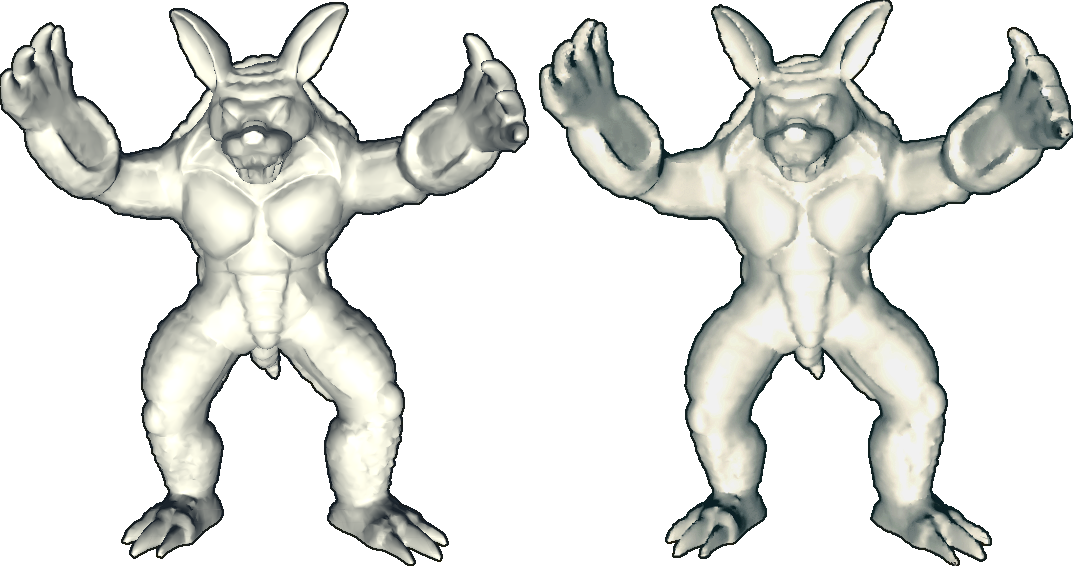
\includegraphics[width=0.75\textwidth]{voxelizer_example_transparent_3.png}
\caption{The Stanford Armadillo mesh\protect\footnotemark  (left) and its voxel representation at a resolution of 128x128x128 voxels (right).}
\label{fig:voxelizer_example}
\end{figure}
\footnotetext{\url{http://graphics.stanford.edu/data/3Dscanrep/}}

An important part of multimedial retrieval is the ability to take query results and reuse them to formulate a new, refined, query. In the context of this thesis the multimedia retrieval
is only concerned with polygonal meshes. To facilitate the modification of such polygonal meshes our application includes a voxelizer module. The voxelizer takes a polygonal
mesh as input and converts it into a suitable voxel representation to enable the user to edit the model volumetrically. Since
our voxels contain not only the voxel material, but also the surface normals, we can reconstruct the mesh from our voxels while keeping most of the mesh's features intact with high accuracy, given
a large enough voxel grid with sufficient resolution. In practice a resolution of 128x128x128 seems to be sufficient for most models that aren't highly detailed or noisy.
Fig. \ref{fig:voxelizer_example} shows an example of a mesh that has been converted to a voxel grid.

\section{Isosurface Polygonization}

Since the voxels are just an internal volumetric representation an algorithm is required to convert them into something that a computer can display on the monitor, e.g. a polygonal 3D mesh. In general these kinds of algorithms are
called isosurface polygonization algorithms, since originally
they were conceived to convert implicit functions, or e.g.
computed tomography (CT) density fields, into a polygonal surface. The word "isosurface" comes from the fact that the implicit function value or density is the same ("iso-", meaning equal) everywhere on the polygonal surface. There are some variants that do not directly work off of density fields but instead some intermediary representation like Hermite data which will be discussed in detail later on.

\begin{figure}
\centering
\captionsetup{width=0.8\textwidth}
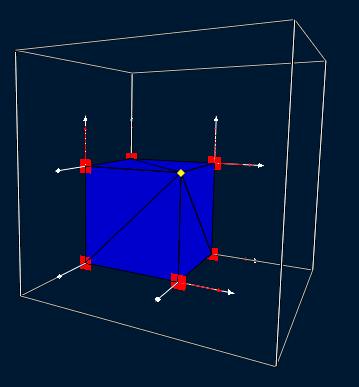
\includegraphics[width=0.35\textwidth]{voxel_scene_cube.png}
\caption{A polygonized voxel cell (white) containing the polygon surface of a cube's corner (blue) with a sharp feature (yellow).}
\label{fig:polygonized_cube_voxel_cell}
\end{figure}

%Method for converting voxels into meshes, some common algorithms as examples

The two main groups of isosurface polygonization alrogithms are the primal (\todoMissing{Missing ref; MC etc.}) and dual (\todoMissing{Missing ref; DC, CMS, etc.}) contouring algorithms.
Most of these algorithms cannot polygonize a single voxel by itself, but instead require a cell consisting of eight voxels, usually arranged in the form
of a cube. Primal and dual contouring algorithms differ in that the primal variants place polygon vertices somewhere on the cell's edges and the dual variants
place them not on the edges but somewhere within the cell's volume. Therefore dual contouring algorithms have the advantage that they can more reliably polygonize
surfaces with sharp features, such as e.g. the corners of a cube. Primal contouring algorithms can also polygonize sharp features in certain cases, however only
if said sharp feature lies exactly on a cell's edge. Fig. \ref{fig:polygonized_cube_voxel_cell} shows a polygonized voxel cell where the sharp feature lies within
the voxel cell.\\
Marching Cubes [\todoMissing{Missing ref}] (MC), a primal contouring algorithm, checks whether the material at each corner of the voxel cell is filled or empty and then 
packs all 8 resulting booleans into a single 8 bit integer. That integer is then used to index into a lookup table that contains which cell edges are to be connected to
each other to form polygons. Vertex positions can either lie on the middle of their respective cell edge or if the voxel contains a density value the vertex position
can be smoothly linearly interpolated.\\
Dual Contouring [\todoMissing{Missing ref}] (DC) uses another approach. A valid voxel cell always contains either no edge with a material, or at least three edges with a material change. If a voxel cell
does contain edges with a material change then Dual Contouring finds the sharp feature that minimizes the squared distance between the sharp feature and all planes spanned
by the normals at the edges with the material changes. In a second pass the generated vertices are then connected between neighboring voxel cells to form polygons.\\
Cubical Marching Squares [\todoMissing{CMS}] (CMS) makes use of both primal and dual contouring features. Much like MC it places vertices on voxel cell edges. However it can also place vertices
on voxel cell faces and within the voxel cell volume, like dual contouring algorithms do. This gives it the advantage that each cell can be polygonized individually while still being able to
reliably polygonize surfaces with sharp features.

\section{CSG}

\begin{figure}
\centering
\captionsetup{width=0.4\textwidth}
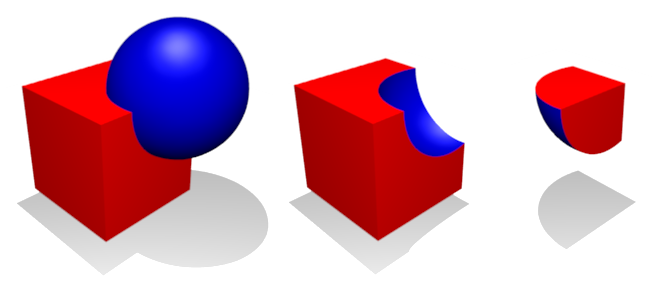
\includegraphics[width=0.4\textwidth]{csg_operations.png}
\caption{Boolean union (left), difference (middle) and intersection (right) of a cube and sphere primitive. Adapted from Wikipedia\protect\footnotemark.}
\label{fig:csg_operations}
\end{figure}
\footnotetext{\url{https://en.wikipedia.org/wiki/Constructive_solid_geometry}}

Constructive Solid Geometry (CSG) is a method to create geometric shapes by constructing them from primitives and a few operations.
The three most common operations are the boolean union ($\cup$), difference ($-$) and intersection ($\cap$) operations are shown in Fig. \ref{fig:csg_operations}. With just
those three simple tools and a couple of primitives, e.g. spheres, cubes, cylinders, etc., the user can easily create arbitrary shapes or sculptures.
Additionally CSG need not be restricted to only boolean operations, but can also make use of smooth operations that blend two shapes together in a continuous
manner. In the context of signed distance functions (see further below) these smooth operations correspond to the smooth minimum and maximum operations.\\
The application developed for this thesis makes extensive use of CSG to enable the users to edit and shape their voxel based sculptures. The union ("add") and
difference ("remove") operations are intuitive and easy to use. Additionally it also provides a "replace" operation that allows the user to replace solid materials inside
a primitive with another material. Logically it is equivalent to $(A-B) \cup (B \cap A)$ where A is the existing sculpture and B is the primitive or bounds within
which solid materials should be replaced with B's material.

\section{Signed Distance Functions}

Signed distance functions (SDF) are mathematical formulas that describe the signed distance between a point and the surface of a certain shape. For points inside the shape the
signed distance is negative. For example it is trivial to derive the signed distance function $f(x,y,z) = \sqrt{x^2 + y^2 + z^2} - r$ of a sphere at $(0, 0, 0)$ from the implicit formula of the sphere's surface, $x^2 + y^2 + z^2 - r^2 = 0$. There exist readily available formulas for SDFs of various shapes, e.g. Inigo Quilez' collection of such functions\footnote{\url{https://iquilezles.org/www/articles/distfunctions/distfunctions.htm}}.\\
SDFs are well suited as a representation of CSG primitives because one can approximate their union and difference by taking the minumum, respectively maximum, of two SDFs. This approach generally works
well and can produce the exact union or difference, however in certain cases it can result in an incorrect approximation, especially on the inside of union'd SDFs. For the purposes of this application the
SDFs need not be exact on the inside, hence we have decided to use SDFs as the representation of our CSG primitives. Additionally since the domain and range are the same for all SDFs, namely
$f\colon \mathbb{R}^3 \mapsto \mathbb{R}$, they can all be treated exactly the same besides their formulas and can be encapsulated as a simple method in code.

%\section{Unity}
%What, why

\section{Architecture}
%How all components are connected to each other (cineast, feature module, cottontail, rest api, polygonizer, voxel storage, vr interaction controller, etc.)

\begin{figure}
\centering
\captionsetup{width=0.8\textwidth}
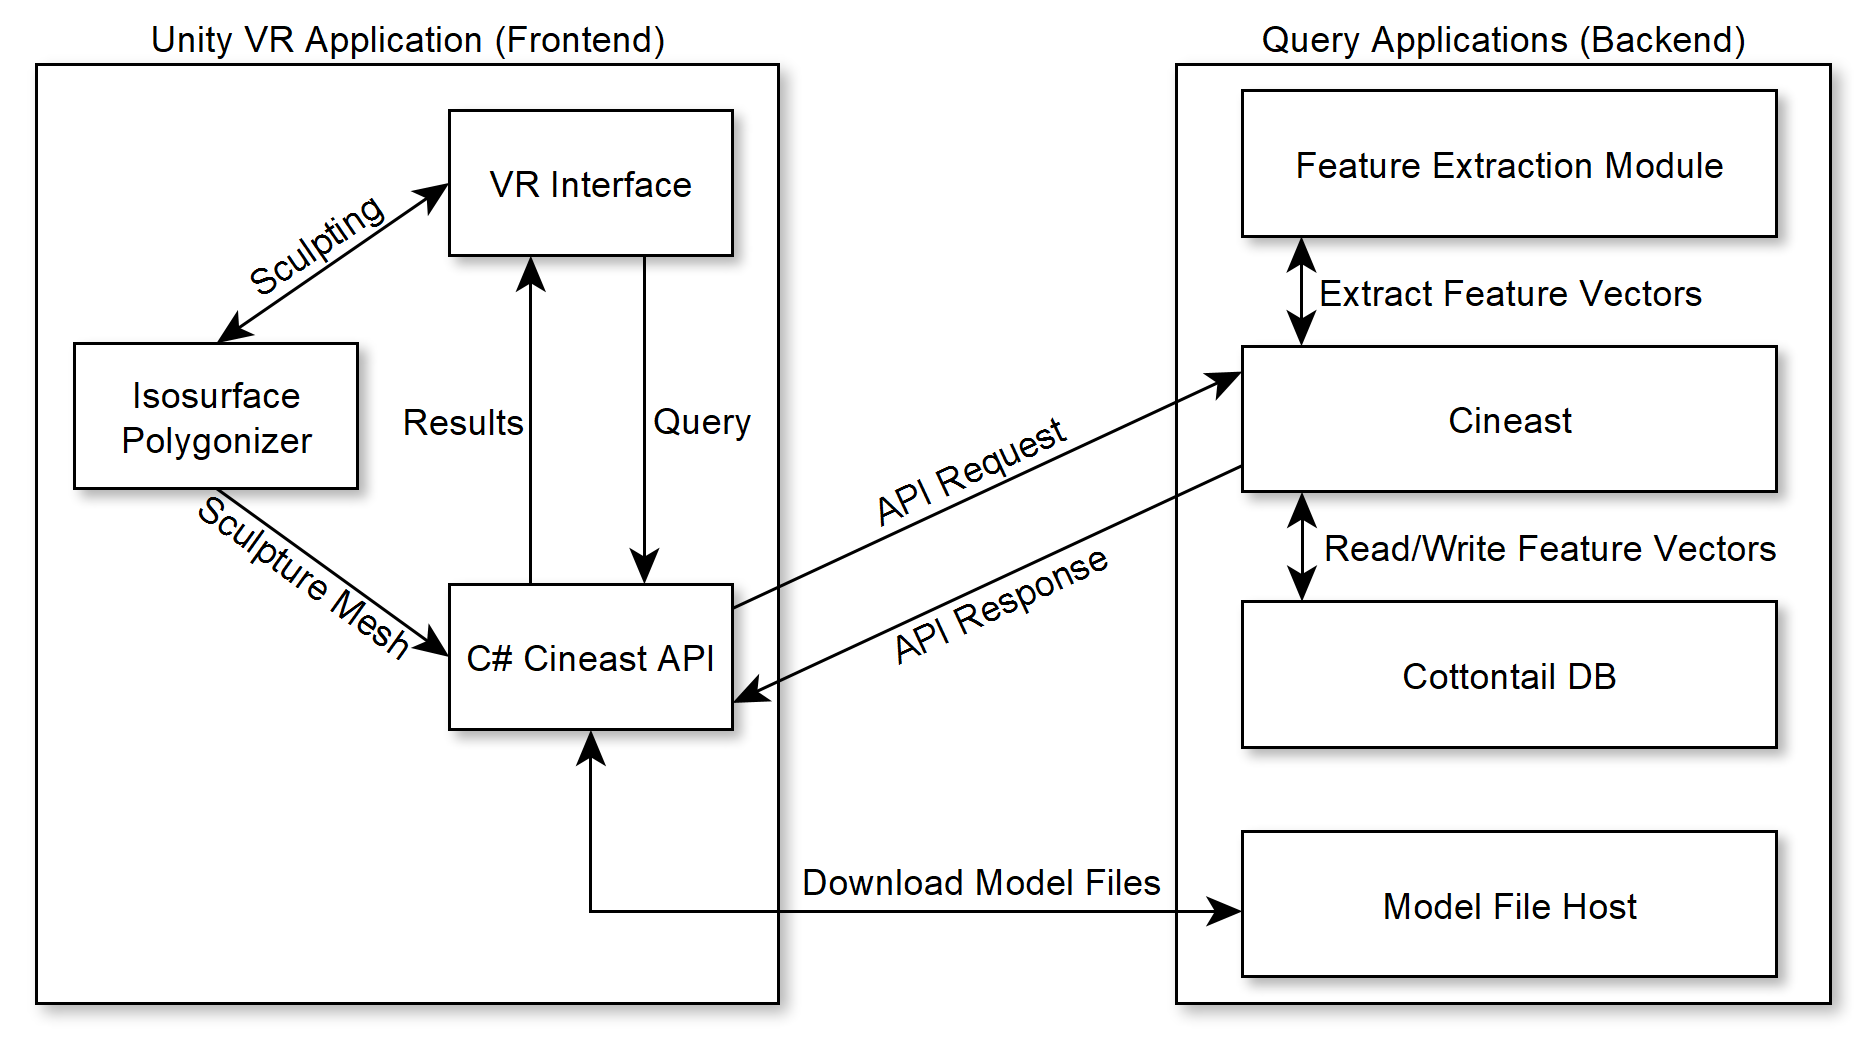
\includegraphics[width=0.8\textwidth]{architecture.png}
\caption{The high level architecture of our system.}
\label{fig:architecture}
\end{figure}

To tie this all together Fig. \ref{fig:architecture} illustrates the high level architecture of our system. The frontend, i.e. our VR application running in the Unity
engine, contains three main components relevant for the querying functionality: the VR interface, isosurface polygonizer and generated C\# Cineast API module.\\
Through the VR interface the user can sculpt using voxels and CSG operations and start queries or view query results. On starting a query from the VR interface the entire sculpture is converted into a single mesh which is then sent to Cineast as an API request via the C\# Cineast API.\\
Cineast then tasks the feature extraction module to convert the mesh into a feature vector. This feature vector is then sent over to the Cottontail DB multimedia database to be
compared with the feature vectors of other models. All models in that multimedia database that have a similar feature vector are then scored, ranked and their IDs are sent back to be received by the C\# Cineast API. The C\# Cineast API then uses the received IDs to download the respective model files and hands them over to the VR interface to be displayed.


\chapter{Implementation}

This chapter goes more into detail about the concepts and architecture mentioned in Chapter \ref{chap:concepts_and_architecture} and how they
are implemented in our application. Text \textsc{in this font} refers to code classes, methods or fields. Method parameter types are specified in the parentheses following the method name.\\
The chapter starts out by elaborating the implementation details about the multimedia retrieval application Cineast and how it was extended to support model similarity queries that take 3D model color and texture into consideration. Furthermore, it explains how our VR sculpting application communicates with Cineast.\\
Following that, it explains how voxels were used to implement the sculpting functionality, sculpture rendering and how the CMS algorithm was extended to support multi-material voxel volumes. In addition to that it presents an algorithm to
convert 3D model meshes into a voxel representation and we propose a new lookup table based implementation of the CMS algorithm.\\
Finally, it ties all these features together and describes how they were combined to form our VR sculpting application.

\section{Cineast}

Cineast is the multimedia retrieval backend of choice for our application. In order to implement the requirements of our application
several changes had to be made to Cineast. However due to Cineast's modular structure most of the changes could be applied without having to
modify the core code.


\subsection{Core Changes}
\label{sec:core_changes}
%UV + texture support in meshes and OBJ loader

Cineast's mesh classes \textsc{Mesh}, \textsc{ReadableMesh} and \textsc{WritableMesh} did not support model textures and thus had to be extended
for our feature module. Methods to get/set a \textsc{BufferedImage} texture and a \textsc{String} texture path, for later retrieving the model texture
through the API, were added to the respective classes. The mesh's \textsc{Vertex} class was also extended to support storing \textsc{Vector2f} texture UV attributes.\\
The \textsc{OBJMeshDecoder}, which is responsible for reading an OBJ-model file into a \textsc{Mesh}, was extended to also read texture UV coordinates.
Moreover, it looks for a texture file with the same name as the OBJ-model file. If such a texture file is found it is added to the \textsc{Mesh} and the texture file's
path is persisted in the database as metadatum with the domain "TEXTURE" and key "texture\_path". To do so the \textsc{Segmenter} class received an additional method
\textsc{persist(SegmentContainer, MediaSegmentDescriptor)} which is called when a \textsc{SegmentContainer} is persisted by \textsc{GenericExtractionItemHandler}.
\textsc{ModelSegmenter} then uses that method to persist the mesh's texture file path metadatum. This metadatum can later be used by clients to download the model's texture.\\
A similar change was required in the \textsc{ModelQueryContainer}. Model data is being sent to Cineast over its REST API, described in Section \ref{sec:rest_api}, in the form of a custom string based model format. This format however does not support vertex colors which are required for color sensitive queries. For this reason a new \textsc{ColorMeshParser} class was added that uses a similar format but also supports vertex colors. Based on the prepended MIME type, an identifier used to describe the format of data, the \textsc{ModelQueryContainer} can decide which parser to use. Like this the API remains backwards compatible with the model format that does not contain vertex color data.\\
Throughout the course of development of this thesis Cineast's REST API was partially rewritten to use the Javalin\footnote{https://javalin.io/} web framework instead of Spark\footnote{http://sparkjava.com/} and SparkSwagger\footnote{https://github.com/manusant/spark-swagger}. Javalin makes great use of Cineast's already built-in JSON serialization structure using Jackson\footnote{https://github.com/FasterXML/jackson}. This enables Javalin, in combination with its OpenAPI plugin,
to generate an OpenAPI specification \cite{openapi} that describes Cineast's REST API in a standardized way. An excerpt of this OpenAPI specification is shown in Listing \ref{lst:openapi_spec} of Section \ref{sec:rest_api}. Since Javalin's OpenAPI plugin makes use of Jackson, it is capable of more reliably creating the specifications for JSON data structures than SparkSwagger, especially for subclasses of superclasses with generic types.

\subsection{Model Formats}

The current implementation supports the Wavefront OBJ format \cite{wavefront_obj} as it is comparatively
simple to parse. However, the feature extraction algorithm is agnostic to the original 3D model format and only requires
a 3D mesh consisting of triangles and vertices that contain the following attributes: position and texture coordinates or vertex colors.
Because of Cineast's modular nature it is possible to add parsers for other 3D model formats, or
to extend the currently existing parsers to also read the aforementioned vertex attributes, without having to alter
the feature extraction algorithm.

\subsection{ClusterD2+Color Feature Extraction}
%What, why (color support), explain assumptions made that were not covered by the paper

Since our application allows the user to color their sculptures it makes sense that our similarity queries for 3D models also
take color into account. Hence part of the color information must be contained in the feature vector, which will then be used
to compare 3D models for similarity as described in Section \ref{sec:multimedia_retrieval_concept}.
Currently, none of Cineast's feature extraction modules take the color of 3D models into consideration.\\
The ClusterD2+Color algorithm \cite{cluster_d2_color}, which was used in our application,
achieves this by creating random sample points on the 3D model's surface according to certain criteria and then
use those sample points to compute a feature vector.\\
Our feature module, \textsc{ClusterD2AndColorHistogram}, extends Cineast's \textsc{StagedFeatureModule} class which takes care of the
querying base functionality, such as searching for similar feature vectors and sorting results by score or persisting an extracted feature vector.
The \textsc{ClusterD2AndColorHistogram} class mostly takes care of extracting the ClusterD2+Color feature vector from a given input model.\\
In order to obtain the data required to construct a feature vector the algorithm runs through the following stages:

\subparagraph{Sample Generation}

Many isosurface polygonization algorithms, such as the non-adaptive CMS implementation used in this application, can produce highly tessellated meshes. On the other hand meshes exported by
3D modeling software are often optimized to have large triangles where the surface has little detail, and small triangles where
the surface is more detailed. Hence it is important that the sample point generation is mostly independent of the triangle sizes
of the mesh, so that meshes of varying levels of tessellation can be compared for similarity effectively.
The ClusterD2+Color algorithm achieves this by making the sampling directly proportional to the surface area of the triangles, hence a sample point
has a higher chance to be positioned on a large triangle, and a smaller chance to be positioned on a small triangle.
Before any sample points are generated the model is first scaled such that its total surface area equals 100.
After generating a certain number of samples, the result is a collection of samples that are uniformly distributed on the mesh's surface. The number of samples
is determined by a function of the integral of the absolute Gaussian curvature over the model's surface as described in \cite{cluster_d2_color}.

\begin{figure}
\centering
\captionsetup{width=0.8\textwidth}
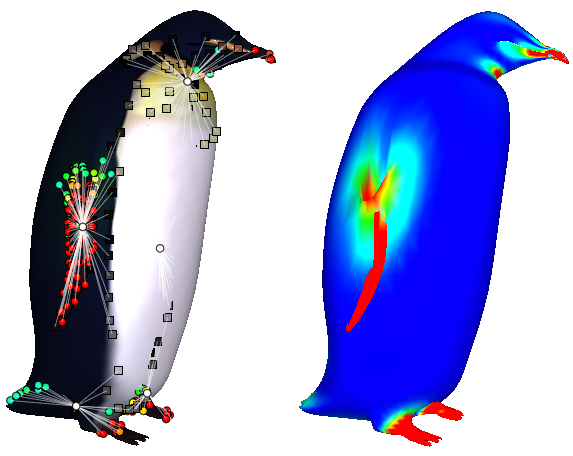
\includegraphics[width=0.5\textwidth]{feature_penguin.png}
\caption{Visualization of the sample selection and clustering. On the left is shown the textured input model and the resulting shape (circles) and color (squares) samples
and their cluster assignments (white circles and lines). The picture on the right shows the computed difference-of-Laplacian $D$ of the model (red: high, blue: low).}
\label{fig:feature_penguin}
\end{figure}

\subparagraph{Shape Sample Selection}

These samples should convey relevant information about the geometric shape. Previous work done by C. H. Lee et al. \cite{mesh_saliency} has
shown that mean curvature is a good indication for visual saliency and thus for comparing geometric shapes for similarity. The mean curvature of the mesh vertices is computed using Taubin's method \cite{taubin_method}.
Our implementation of the ClusterD2+Color algorithm computes the mean curvature of each vertex and stores it as a vertex attribute. This mean curvature attribute is then smoothed over the mesh's surface
by a Laplacian smoothing approximation described in \cite{implicit_fairing}, resulting in a curvature map.
In particular, our implementation sets $\lambda = 8$ and, to satisfy the stability criterion $\lambda dt \leq 1$, $dt = \frac{1}{8}$, i.e. equivalently it applies small smoothings with $\lambda = 1$, $dt = 1$ a total of eight times for one
full smoothing operation. This is repeated multiple times to create three smoothed curvature maps $C^1$ through $C^3$. Each curvature map $C^i$ has been smoothed $i$ times.

\begin{figure}
\centering
\captionsetup{width=0.8\textwidth}
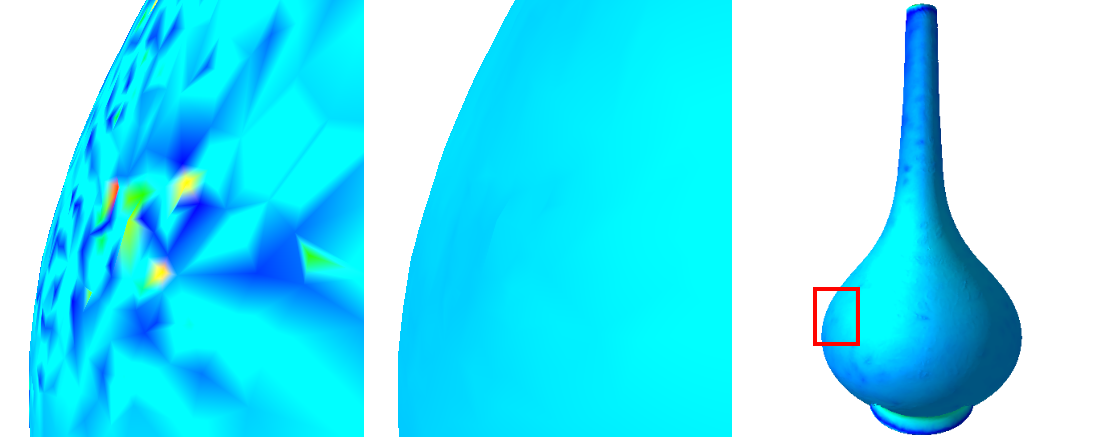
\includegraphics[width=0.6\textwidth]{laplacian_smoothing_artefacts_transparent.png}
\caption{$C^0$ (left) exhibits significant artefacts on a non-manifold vase mesh (right) which has many invisible touching edges. $C^1$ (middle) is a more sensible curvature map as baseline for the shown model.}
\label{fig:laplacian_smoothing_artefacts}
\end{figure}

As opposed to \cite{cluster_d2_color} we use
$C^1$ as the baseline curvature map instead of $C^0$, because certain non-manifold models exhibit significant artefacts in $C^0$ as illustrated in Fig. \ref{fig:laplacian_smoothing_artefacts}. A mesh is considered non-manifold when it has unconnected vertices or edges that are touching. Lastly each shape sample calculates its $D = D^2 \oplus D^3$ value, where $D^i = C^i - C^{i-1}$ is the difference-of-Laplacian space, as depicted in Fig. \ref{fig:feature_penguin}, and only the samples with the top 10\% highest $D$ values are kept. Indeed the remaining top
10\% $D$ value shape samples in Fig. \ref{fig:feature_penguin} are concentrated to the relevant features of the penguin model, namely its arms, feet and beak.

\subparagraph{Color Sample Selection}

The color samples' purpose is to allow the algorithm to distinguish between models that have the same geometric shape but differ in
color or texture. This is achieved by only selecting those samples that lie on significant color transitions. As described by
Y.-J. Liu et al. \cite{cluster_d2_color}, all generated samples extract the mesh's color at their position and then transform
the color to the CIE-LAB color space \cite{cie_color_space}, which aims to provide a perceptually uniform color space, i.e. same distances in CIE-LAB color space correspond to the same amount of perceptual difference.
The resulting three CIE-LAB coordinates, $L^*$, $a^*$ and $b^*$ are then quantized into 6 ($L^*$), respectively 4 ($a^*$) and 4 ($b^*$) integer values. These three, now quantized, coordinates are combined into a single color code integer, such that each of those color codes corresponds to a unique combination of the quantized coordinates. Perceptually similar colors are thus mapped to the same color code and dissimilar colors are mapped to different color codes.\\
Lastly the algorithm only selects those samples as color samples of which less than $80\%$ of the neighboring samples' color codes are the same. In our implementation the neighborhood range is defined as a function of the model's mean edge length, or if less than 5 samples are found within said range then it chooses the 5 nearest samples as the neighborhood. In Fig. \ref{fig:feature_penguin} the
color samples are selected mostly along the transition between the white, black and beige hair of the penguin

\subsection{Comparing Features For Similarity}
%L2 norm, Jensen-Shannon divergence, $\chi^2$ distance

The selected shape and color samples now need to be reduced into an N-dimensional feature vector. ClusterD2+Color algorithm achieves this by first clustering nearby samples together and then
creating a histogram from the euclidean distances, i.e. L2 norm, between all samples that are not in the same cluster.\\
More specifically, the samples are clustered together using a modified
ISODATA algorithm described in \cite{cluster_d2_color}. In our implementation we set $P_n = 5\%$ \textit{of the total number of sample points}, $P_s = 2 * E$, $P_c = 10 * E$, $I = 100$ with $E =$ \textit{mean edge length of the model}.
Additionally we introduce two new parameters: $I_{min} = 10$, the minimum number of iterations, and $I_{nc} = 200$, the total maximum number of iterations after which the algorithm is stopped if no convergence is happening. Without
the $I_{min}$ parameter we have observed that the algorithm would commonly stop too early with inadequate cluster assignments. Then, once the samples are clustered together, the euclidian distances between all samples in different clusters
are computed and stored in an array. The values in this array are then normalized such that the lowest value in the array is mapped to zero and the highest value is mapped to one. Finally this array is then converted into a histogram with $20$ bins.\\
Y.-J. Liu et al. \cite{cluster_d2_color} have also proposed a second method called ClusterAngle+Color which calculates the values for the histogram from the angle between triplets of samples that are each in different clusters. According
to the authors this method results in a better similarity measure, however due to the $O(N^3)$ complexity we have unfortunately found it to be infeasible with the large number of samples generated from the user sculpted models in our application.\\
In either case the result is a histogram which serves as 20-dimensional feature vector and in fact, since they are a geometric signature of the model, they can be used to compare models for similarity,
e.g. by using the $\chi^2$ distance metric, a commonly used distance metric to compare two histograms for similarity. The lower the $\chi^2$ distance the more similar the models. Conveniently Cineast and its multimedia retrieval
database Cottontail DB offer an efficient k-nearest neighbors query for the $\chi^2$ distance metric.\\

\begin{figure}
\centering
\captionsetup{width=0.8\textwidth}
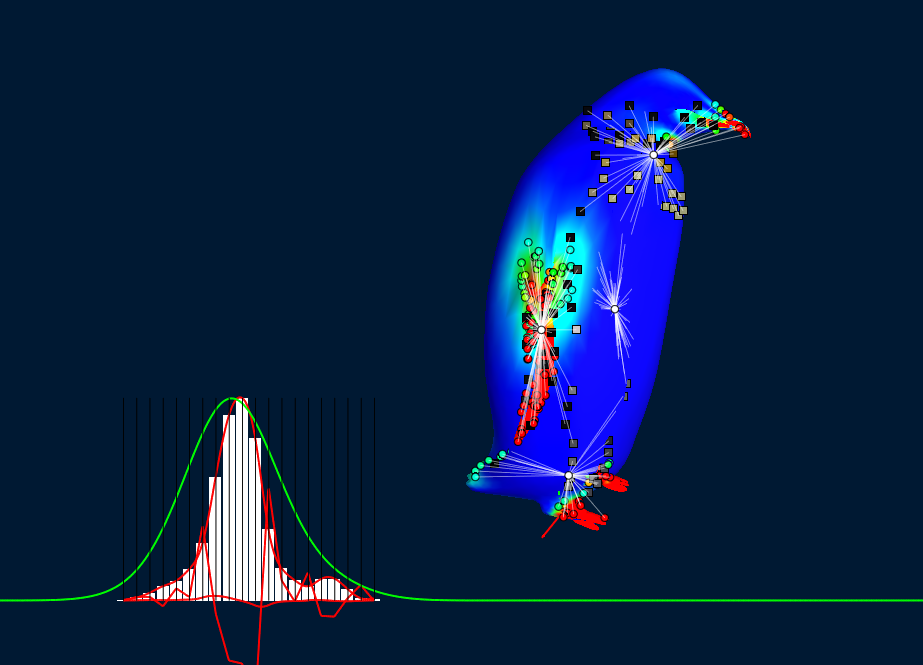
\includegraphics[width=0.5\textwidth]{feature_penguin_histogram.png}
\caption{The feature visualization tool that was developed during the feature extraction implementation. White: histogram feature vector. Green: probability density function of the histogram.}
\label{fig:feature_penguin_histogram}
\end{figure}

Along with the $\chi^2$ distance metric the Jensen-Shannon divergence ($D_{JS}$) was implemented. This is the metric Y.-J. Liu et al. \cite{cluster_d2_color} chose for their implementation. In short, the $D_{JS}$ metric treats the histogram feature vector as an independent and identically-distributed sample of a random variable and thus first converts the histogram into a probability density function by using kernel density approximation with a gaussian kernel. The Jensen-Shannon divergence of the two probability density functions to compare is then computed and serves as a probabilistic measure ranging from 0 to 1 for how similar they are, so in a sense how likely it is that the two histograms were generated from the same model. Fig. \ref{fig:feature_penguin_histogram} depicts the histogram of a penguin model and its probability density function, along with some debug information of curves required for the $D_{JS}$ calculation.\\
In our ClusterD2+Color implementation in Cineast $D_{JS}$ is currently significantly slower than $\chi^2$ because Cottontail DB does not natively support k-nearest neighbors queries for $D_{JS}$. Therefore Cineast must retrieve the feature vectors of all currently existing models in the database and compare all of them one by one to the input feature vector using $D_{JS}$.\\
The exact reason why Y.-J. Liu et al. used the Jensen-Shannon divergence was not mentioned, other than the fact that for a given 3D model they "[...] regard its shape histogram as an independent and identically-distributed sample of a random variable [...]" and thus convert it to a probability density function which can be compared using $D_{JS}$. We speculate that $D_{JS}$ may be more robust to noise from the random sample generation than the $\chi^2$ distance metric due to the conversion to a smooth probability density function. However this may incur a slight general loss of accuracy due to the smoothing.\\
Finally Cineast can run multiple features or distance metrics for a single query and then combine their scores by weights specified in Cineast's configuration. This can be useful to capture different kinds of feature types in a single similarity score.


\subsection{C\# Cineast API}
\label{sec:rest_api}

Cineast provides two main APIs, a WebSocket API and more importantly a REST API which was used for the purposes of this thesis. The operating principles of a REST API are described in Section \ref{sec:rest_api_concept}.\\
For example Cineast's similarity query endpoint is executed by sending a \textit{POST} request to \url{http://cineast.domain/find/segments/similar}. Additional data, such as the model to run the similarity query for, is included in the HTTP request body in the form of JSON data as specified in "requestBody" of Listing \ref{lst:openapi_spec}. The structures of the used schemas are not shown in the listing but they are specified in the same file.

\begin{mdframed}[
	backgroundcolor=light-gray,
	roundcorner=10pt,
	leftmargin=1,
	rightmargin=1,
	innerleftmargin=25,
	innertopmargin=0,
	innerbottommargin=0,
	outerlinewidth=1,
	linecolor=light-gray
]
\lstset{style=json}
\begin{lstlisting}[
	caption={Part of the Cineast OpenAPI specification responsible for the similarity query API endpoint.},
	label=lst:openapi_spec
]
"/find/segments/similar": {
 "post": {
  "tags": ["/api/v1"],
  "summary": "Finds similar segments based on the given query",
  "description": "Finds similar segments based on the given query",
  "operationId": "FindSegmentSimilarActionHandler#POST",
  "requestBody": {
    "content": {
     "application/json": {
     "schema": {
      "$\dollar$ref": "#/components/schemas/SimilarityQuery"
     }
    }
   }
  },
  "responses": {
   "200": {
    "description": "OK",
    "content": {
     "application/json": {
      "schema": {
       "$\dollar$ref": "#/components/schemas/SimilarityQueryResultBatch"
      }
     }
    }
   }
  }
 }
}
\end{lstlisting}
\end{mdframed}

The OpenAPI specification mentioned in Section \ref{sec:core_changes} allows programs like Swagger Codegen\footnote{https://swagger.io/tools/swagger-codegen/} to generate fully functional code libraries in various programming languages capable of interfacing with the REST API defined by the specification. The C\# library that was used to access Cineast's API endpoint from Unity was generated by Swagger Codegen from Cineast's OpenAPI specification.

\begin{mdframed}[
	backgroundcolor=light-gray,
	roundcorner=10pt,
	leftmargin=1,
	rightmargin=1,
	innerleftmargin=25,
	innertopmargin=0,
	innerbottommargin=0,
	outerlinewidth=1,
	linecolor=light-gray
]
\lstset{style=sharpc}
\begin{lstlisting}[
	caption={Calling the generated C\# code of the similarity query API endpoint.},
	label=lst:csharp_cineast_api_call
]
var terms = new List<QueryTerm> {
 new QueryTerm {
  Categories = categories,
  Type = QueryTerm.TypeEnum.MODEL3D,
  Data = "data:application/3d-color-json," + base64ModelData
 }
};
var components = new List<QueryComponent> {
 new QueryComponent {
  Terms = terms
 }
};
var conf = new QueryConfig();
var query = new SimilarityQuery {
 Components = components,
 Config = conf
};
var response = await Api.FindSegmentSimilarActionHandlerPOSTAsync(query);
\end{lstlisting}
\end{mdframed}

Listing \ref{lst:csharp_cineast_api_call} shows an excerpt from our code that sends Cineast a similarity query REST request by calling the Swagger Codegen generated C\# method \textsc{FindSegmentSimilarActionHandlerPOSTAsync} and using the generated classes \textsc{QueryTerm}, \textsc{QueryComponent}, \textsc{QueryConfig} and \textsc{SimilarityQuery}.

\section{Hermite Data Voxels}

\begin{figure}
\centering
\captionsetup{width=0.8\textwidth}
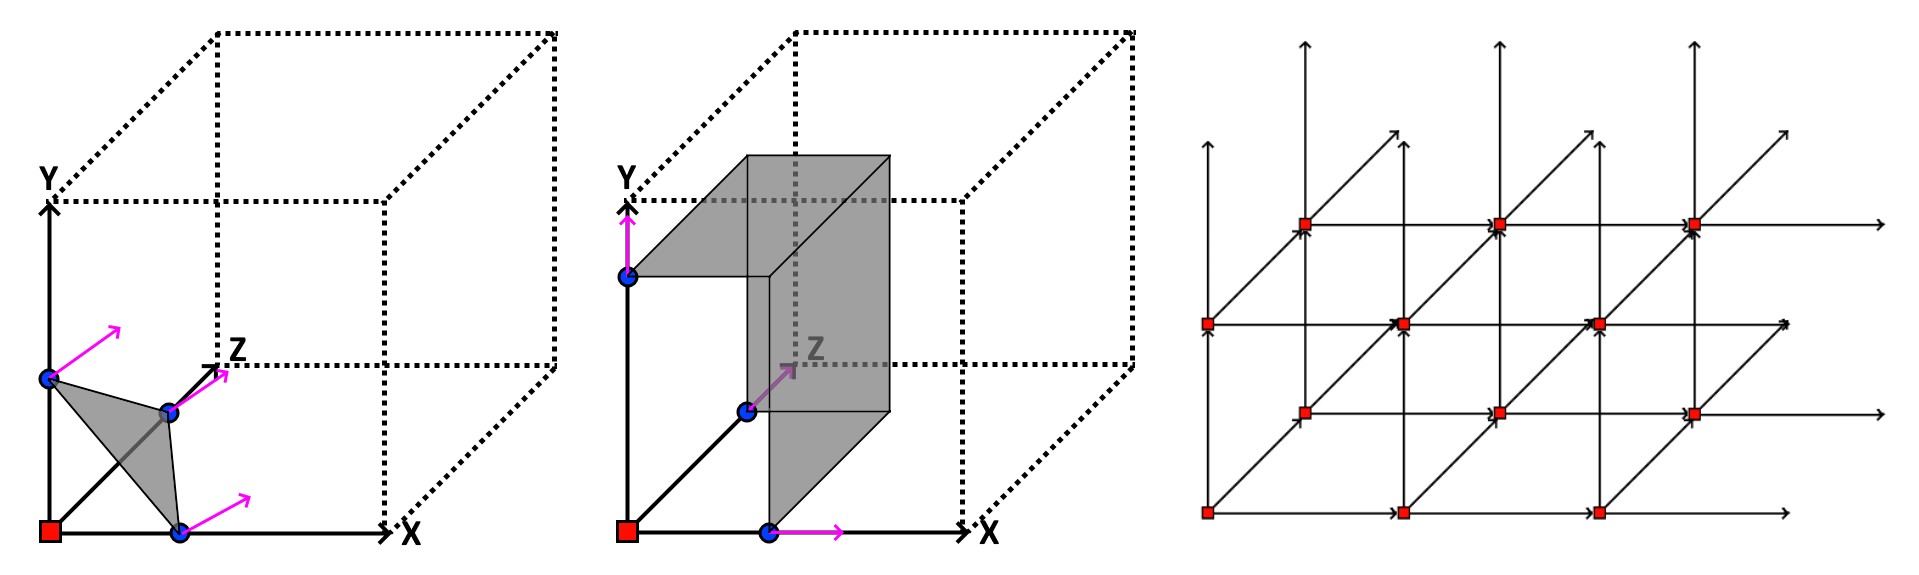
\includegraphics[width=\textwidth]{hermite_data_2.png}
\caption{Hermite data voxels. One Hermite data voxel contains 1 material ID (red squares), up to three intersection points (blue circles) and their respective normals (pink arrows). Depending on the configuration of
the intersection points and normals one voxel can take various shapes (gray areas), e.g. a single triangle (left) or a sharp corner (middle). The Hermite data voxels can be arranged in a grid (right) to form closed surfaces.}
\label{fig:hermite_data}
\end{figure}

Since voxels are an abstract representation of volumes they can be visualized in various ways depending on the data the voxel contains.
Originally a voxel consisted of a single attribute, a color or binary solid/non-solid, in which case the voxel can be visualized for example by cubes, spheres or splats.
More sophisticated voxels can contain additional attributes such as normals or texture coordinates and thus can have a different look based on these attributes.\\
In particular, our application uses voxels that consist of a 32 bit material ID plus Hermite data \cite{dual_contouring}. Hermite data, first used for voxels in \cite{dual_contouring},
consists of the following attributes: exact intersection points and normals. This allows the voxel to take on various shapes much like MC, but with more precision since the exact intersection points are stored explicitly and
sharp features can be constructed from the stored normals. Fig. \ref{fig:hermite_data} illustrates the Hermite data and how it can represent diverse shapes. When arranged in a grid these Hermite data voxels form closed surfaces
like in Fig. \ref{fig:voxel_scene}.
%The Hermite data and voxel material provide enough information to construct the piece of surface represented by a voxel in the form of polygons.

\begin{figure}
\centering
\captionsetup{width=0.8\textwidth}
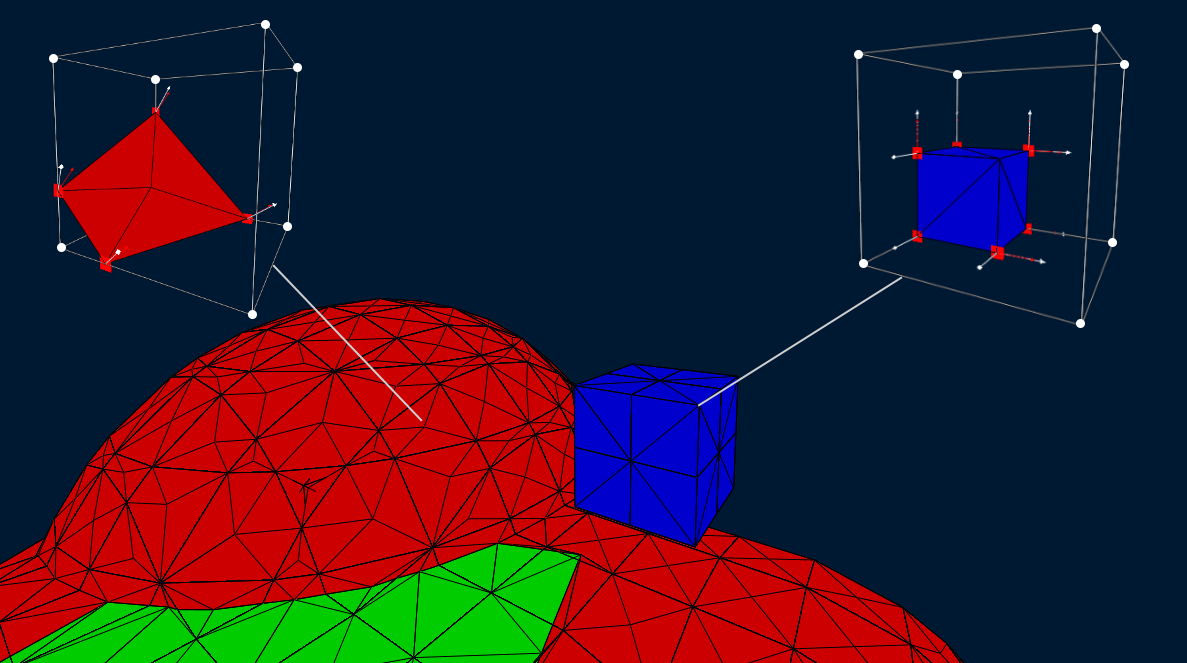
\includegraphics[width=\textwidth]{voxel_scene.png}
\caption{A voxel scene showing the mesh resulting from a grid of Hermite data voxels. Two voxel cells (top left and right) consisting of eight voxels each are shown seperately to highlight how
the mesh is constructed by combining the partial surfaces of al voxel cells. Colors signify different materials.}
\label{fig:voxel_scene}
\end{figure}

\subsection{Voxel Storage}

\begin{figure}[!htb]
\minipage{0.49\textwidth}
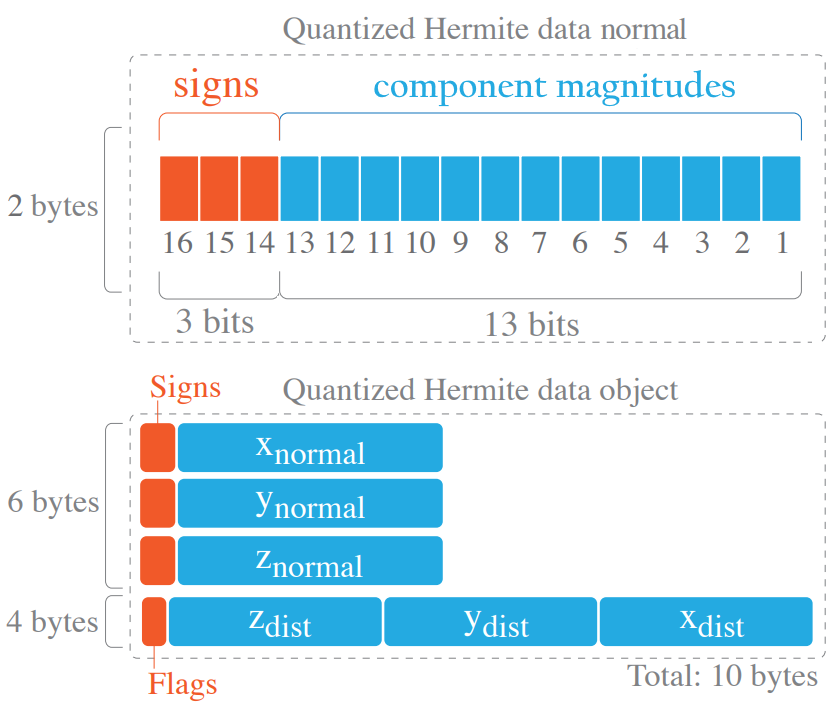
\includegraphics[width=\linewidth]{quantized_hermite_data.png}
\caption{Quantized Hermite data structure. Top: a normal's component magnitudes are packed into 13 bits plus 3 bits for the signs. One normal thus fits into two bytes. Bottom: the entire quantized Hermite data object. $x,y,z_{dist}$ refer to the intersection points. Adapted from \cite{quantized_hermite_data}, pages 18 and 20.}
\label{fig:quantized_hermite_data}
\endminipage\hfill
\minipage{0.49\textwidth}
\vspace*{10mm}
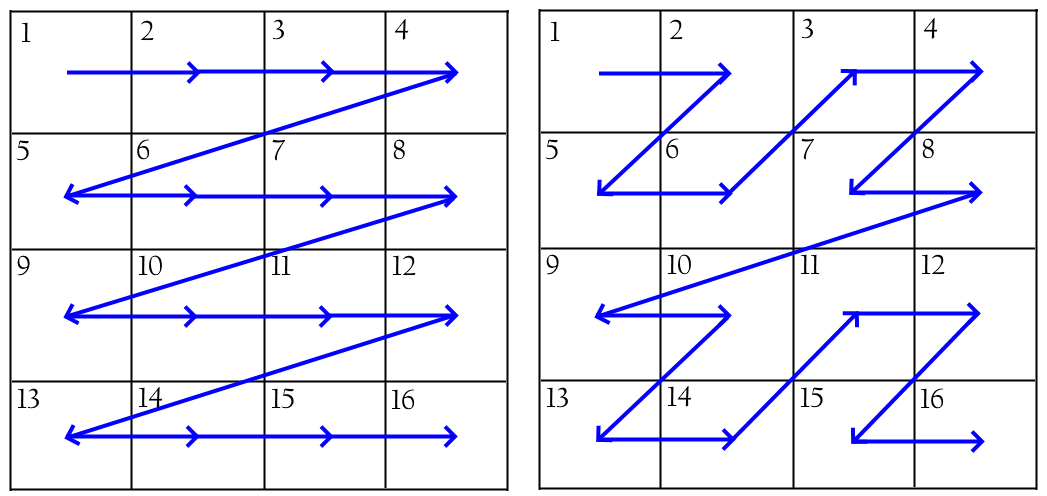
\includegraphics[width=\linewidth]{indexing_order.png}
\vspace*{4mm}
\caption{Simple linear indexing (left), Z-Order indexing (right). Each square represents a voxel in a 2D array. The blue line represents the order in which they are stored in main memory.}
\label{fig:indexing_order}
\endminipage\hfill
\end{figure}

\subparagraph{Data Structure}

There are many different data structures to store voxels, the simplest of which is simply storing the voxels' values in large 3D arrays.
Other data structures however need not necessarily store all voxel values on a regular grid. Often there are regions with many voxels of the same value, and
in that case it is beneficial to use a more advanced data structure that can store voxel values more memory efficiently.\\
The most common method to store voxels in memory is to split the voxels into fixed size blocks or chunks. Within each chunk the voxels are stored in an array. The chunks are stored seperately in a sparse data structure, e.g. a hash map,
where they can be accessed by their position. This gives a good trade-off between memory usage and access speed, because often voxel accesses happen within the same chunks and hence the hash map lookups can usually be cached. Instead of multi-dimensonal arrays for the chunk voxel storage we use one contiguous linear array per chunk to avoid having to dereference multiple pointers for a single access. The index into this linear array can be directly computed from a given X, Y and Z position within the chunk by the following formula: $index(x, y, z) = x * N * N + y * N + z$, where $N$ is the chunk size.
Our implementation uses a chunk size of $N=32$. Voxels on the faces towards the positive X, Y and Z axes are padding voxels that always mirror the state of the neighbor voxel in the respective neighbor chunk.
These padding voxels allow the voxel polygonizer to run faster since it entirely removes the need to query neighbor chunks during meshing. This method is described by \cite{voxel_acceleration} in more detail.

\subparagraph{Memory Consumption}

The voxels in this application consist of a 32 bit material ID plus Hermite data. Therefore the size of a single voxel in memory is: 4 (material) + $3*3*4$ (three normals, each with three 32 bit float components) + $3*4$ (three intersection points) = 52 bytes in total. Considering that a single chunk contains $32 * 32 * 32 = 32768$ voxels, hence consumes roughly 1.7MB, and one scene can contain many of these chunks,
the main memory will be exhausted rather quickly.
To remedy this issue the Hermite data compression scheme described in \cite{quantized_hermite_data} was used.
This quantized Hermite data compression is lossy since it relies on quantizing the floating point values into small integers that are then packed together using bitwise operations. The errors introduced by the compression are
negligible: the exact intersection points remain accurate to a $\frac{1}{1024}$th, respectively less than 0.1\%, of the voxel's edge length. Similarly the maximum error in a normalized normal's component is $\frac{1}{1024}$.
The effective size of the quantized Hermite data is 12 bytes, two of which are struct alignment padding, i.e. only 23\% of the uncompressed size. Fig. \ref{fig:quantized_hermite_data} illustrates the quantized Hermite data
structure in more detail.

\subparagraph{Access Optimization}

When a program accesses a piece of memory from main memory the CPU loads the surrounding address space into one or multiple fixed size cache lines, contiguous pieces of the heap memory around the access, into the cache.
If the program then accesses a nearby address again the CPU can read the value from the cache which is a lot faster than reading it from main memory. This is called a cache hit. On the other hand if the program accesses an address too far away from the previous access or not cached then the CPU will have to read the value from main memory instead, ergo a cache miss. Hence by optimizing for cache hits a program's speed can be improved if it is memory bound. The most
common access pattern for our voxel storage is to read eight neighbor voxels as a voxel cell for polygonization.
For simplicity's sake we will consider a 2D instead of 3D array: if we use simple linear indexing as illustrated in Fig. \ref{fig:indexing_order} to read the voxel cell (1, 2, 5, 6) there will be a large address difference between the voxels
on the first and second row. With large arrays this will often lead to cache misses. By instead using Z-Order indexing, also known as Morton indexing, spacially nearby voxels are much more likely to be nearby to each other in the address space, increasing the chance for cache hits. However, such indexing schemes usually have a larger overhead due to the calculation of the index. To compute the Z-Order indices parts of the Libmorton library\footnote{\url{https://github.com/Forceflow/libmorton}} were used and ported to C\#. Unfortunately in our case using Z-Order indexing has made no significant difference.


\subsection{Cubical Marching Squares}
\label{sec:cms}

\hfill

\begin{figure}[!htb]
\minipage{0.49\textwidth}
\vspace*{10mm}
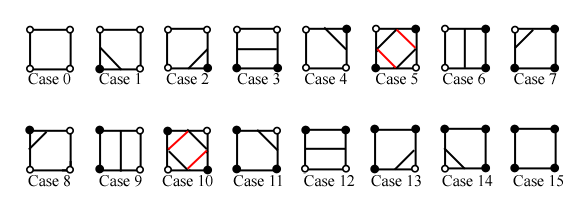
\includegraphics[width=\linewidth]{marching_squares_cases.png}
\vspace*{10mm}
\caption{All marching squares cases. Red lines indicate an ambiguous case,
i.e. either pair of lines is valid if only the corner values of the cell
are available. Source: \cite{marching_squares}}
\label{fig:marching_squares_cases}
\endminipage\hfill
\minipage{0.49\textwidth}
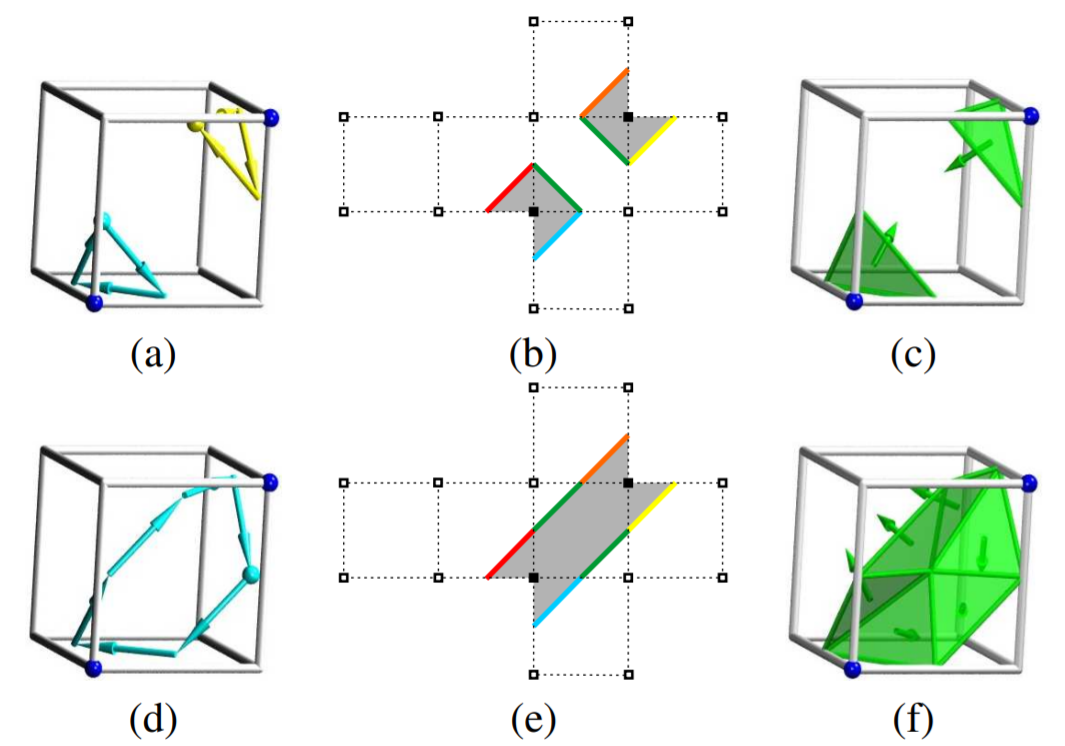
\includegraphics[width=\linewidth]{cms_visualization.png}
\caption{Cubical Marching Squares voxel cell components (a, d), their Marching Squares cell faces (b, e) and their triangulations (c, f). Source: \cite{cubical_marching_squares}, page 3}
\label{fig:cms_visualization}
\endminipage\hfill
\end{figure}

For our application we have decided to use the Cubical Marching Squares algorithm \cite{cubical_marching_squares} to polygonize our voxels. The reason for this choice was
that CMS provides both primal and dual features. As such each cell can be polygonized independently but it can still also preserve sharp features well, e.g. the top of a voxel pyramid.\\
Our implementation of the CMS algorithm runs only on regular voxel grids and
there is no adaptivity or level of detail. Therefore all future explanations on CMS are based on these two limitations.\\
The first step of the CMS algorithm is to run the Marching Squares (MS) algorithm, the 2D counterpart of the MC algorithm, on each face of a voxel cell. Fig. \ref{fig:marching_squares_cases} gives an overview over the total 16 different MS cases for a single voxel cell face. If the normals of the Hermite data span an angle greater than the 2D sharp feature angle threshold then the straight line segments are replaced with two lines that connect the two edges and the intersection point of the normals' tangents. This allows CMS to preserve sharp features on the voxel cell faces. Furthermore this sharp feature helps CMS to resolve the ambiguous MS cases 5 and 10, because the two line segments must not overlap. With the two sharp features in cases 5 and 10 it is simple to check
whether the two sharp segments overlap or not, and then use the non-overlapping configuration.\\
Once all six voxel cell faces have been processed by MS the CMS algorithm connects or links all touching line segments together. The result of this is a collection of components, i.e. groups of line segments that form a loop.\\
Then, for each component in a voxel cell, and all their line segments, CMS outputs vertices. Additionally for each component in a voxel cell, if the component's normals of a component span an angle greater than the 3D sharp feature angle threshold the CMS algorithm finds the component's 3D sharp feature that minimizes the sum of squared distances between the sharp feature and the planes spanned by the component's normals. Then it places a vertex at said sharp feature. If the angle threshold is not met then CMS instead places a vertex at the mean position of the component's vertices. This results in a list of triangles for each component, like illustrated in Fig. \ref{fig:cms_visualization}, that are added to the output mesh.




\subsubsection{Multi-material Extension for CMS}
\label{sec:multi_material_cms}

\begin{figure}
\centering
\captionsetup{width=0.8\textwidth}
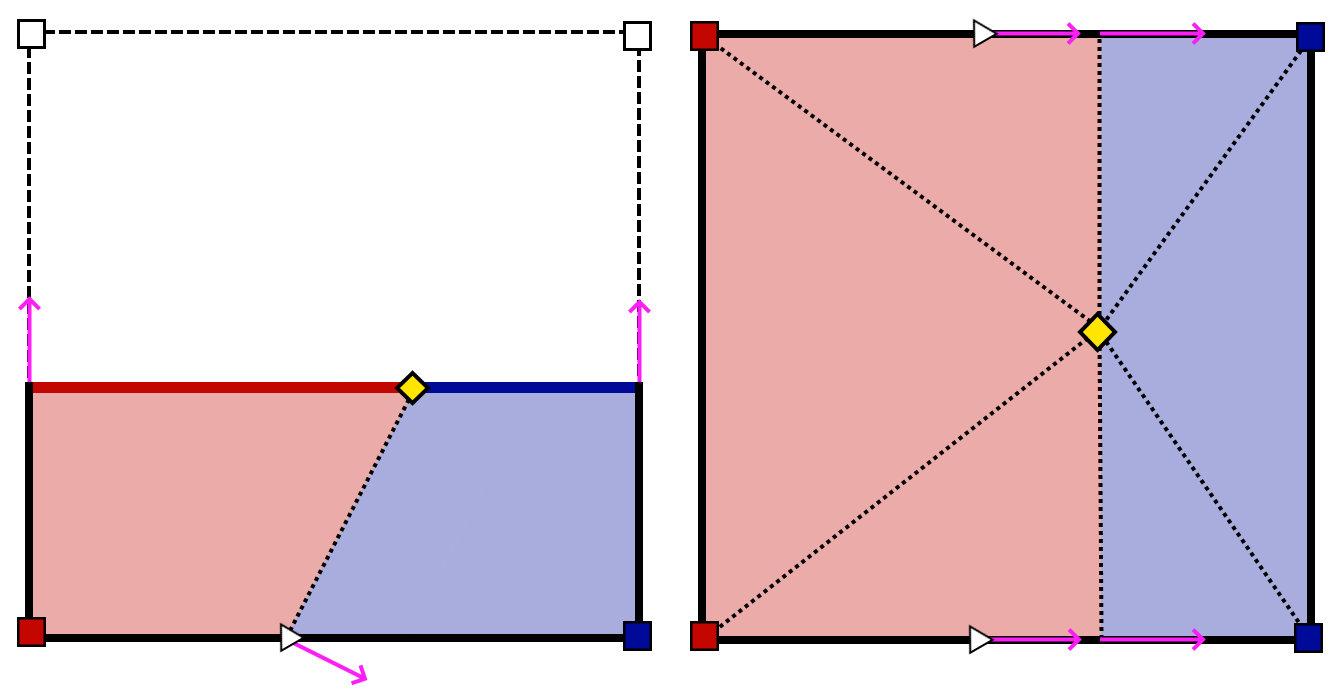
\includegraphics[width=0.5\textwidth]{cms_multi_material_side_top.png}
\caption{Multi-material CMS. The side view (left) shows how the material transitions (white triangles) are projected onto the segment, causing a split where one would expect the material transition to occur on the surface. The top view (right) illustrates how those splits are included in the sharp feature (yellow diamond) solution. The right side also shows the resulting triangulation (dotted lines).}
\label{fig:cms_multi_material}
\end{figure}

\begin{algorithm}[H]
\caption{\textbf{GenerateSegment.} \textit{This procedure remains mostly the same as described in the CMS paper. The only difference is the last line \ref{algstatement:cms_generate_segment_change}.}}\label{alg:cms_generate_segment}
\begin{algorithmic}[1]
\Procedure{GenerateSegment}{Face $f$}
	\If{there are two segments}
		\State $\{l_1, l_2\} \gets $\Call{ResolveFaceAmbiguity}{$f$}
		\State $f.list \gets \{l_1, l_2\}$
		\State \Call{DetectFaceSharpFeature}{$f.list$}
	\ElsIf{there is one segment l}
		\State $f.list \gets \{l\}$
		\State \Call{DetectFaceSharpFeature}{$f.list$}
	\EndIf
	\State \Call{DetectMaterialTransition}{$f$} \label{algstatement:cms_generate_segment_change}
\EndProcedure
\end{algorithmic}
\end{algorithm}

\begin{algorithm}[H]
\caption{\textbf{DetectMaterialTransition.} \textit{This procedure finds and inserts material transitions into the segments of a face f. \textsc{InsertTransition} inserts the transition points into $f.list$ at their appropriate indices s.t. the segment's pieces remain straight and don't form folds, i.e. s.t. they subdivide the segment, and $transition2$ is to be inserted after $transition1$. The MATERIAL\_TRANSITIONS table returns one or two edges connecting two neighboring face corners with solid materials given the marching squares case, since those could contain material transitions.}}\label{alg:cms_detect_material_transition}
\begin{algorithmic}[1]
\Procedure{DetectMaterialTransition}{Face $f$}
	\If{$f.marchingSquaresCase \in \{3,6,7,9,11,12,13,14\}$}
		\State $edges \gets $ MATERIAL\_TRANSITIONS[$f.marchingSquaresCase$]
		\ForAll{$edge \in edges$}
			\State $normal \gets $\Call{GetNormal}{$f, edge$}
			\If{$normal \neq \varnothing$} \Comment{There can only be a transition if a normal exists.}
				\State $intersection \gets $\Call{GetIntersection}{$f, edge$}
				\State $tangent \gets $\Call{ConstructTangent}{$intersection, normal$}
				\ForAll{$l \in f.list$}
					\ForAll{$p \in l$} \Comment{The variable $p$ is one piece of the segment $l$.}
						\If{$tangent$ intersects with $p$}
							\State $transitionPoint \gets $\Call{IntersectionPoint}{$tangent, p$}
							\State $transition1 \gets $\Call{CreateTransition}{\null}
							\State $transition1.position \gets transitionPoint$
							\State $transition1.material \gets edge.points[0].material$
							\State $transition1.normal \gets normal$
							\State $transition2 \gets $\Call{CreateTransition}{\null}
							\State $transition2.position \gets transitionPoint$
							\State $transition2.material \gets edge.points[1].material$
							\State $transition2.normal \gets normal$
							\State \Call{InsertTransition}{$f.list, transition1, transition2$}
						\EndIf
					\EndFor
				\EndFor
			\EndIf
		\EndFor
	\EndIf
\EndProcedure
\end{algorithmic}
\end{algorithm}


The regular CMS algorithm does not support multiple materials. Hence due to the need for multi material volumes in this thesis's application
a multi-material CMS extension was developed. In order for this to work the Hermite data normals must additionally also be stored for each material change edge, and not only for non-solid
to solid changes or vice versa. Furthermore each segment vertex must store a material.
Only one change was required in the algorithms presented in the CMS paper: \textsc{GenerateSegment}'s modification is shown in Alg. \ref{alg:cms_generate_segment}.
Since our application only uses regular voxel grids the modification was made to work on regular voxel grid cells. It can however be extended to work with the adaptive CMS version
in a similar manner.

Additionally to the \textsc{GenerateSegment} modification the \textsc{DetectSharpFeature} implementation also requires a change. The transitions generated in \textsc{DetectMaterialTransition}, which are added to
$f.list$, and their normals must be included in the linear system of equations to be solved \cite{cubical_marching_squares} for the sharp feature detection,
as suggested in \cite{dual_contouring}. This causes the sharp feature to be placed where one would expect the material transition to occur on the surface, as illustrated in Fig. \ref{fig:cms_multi_material}.
This of course means that the multi-material CMS algorithm must always generate a sharp feature when material transitions are present, even if the sharp feature conditions/heuristics described by Kobbelt et al. \cite{kobbelt_sharp_features} , which are used in CMS, are not met.

\subsubsection{Lookup Table Based Implementation}

Much of the CMS algorithm can be done and perhaps be sped up using appropriate lookup tables, especially in the case of regular grid voxel cells. We have generated such lookup tables in order to show
the viability of such an approach. Due to time constraints and it breaking the multi-material extension from Section \ref{sec:multi_material_cms} however, it has ended up not being used in the final implementation.
Nevertheless with some more work it can also be made to work with multi-material volumes. Furthermore this lookup table based approach may prove useful for a future GPU based implementation as it splits
the problem into several small steps that can all be run in parallel with very little divergent behaviour.\\
A tool was implemented to generate the lookup tables for all $2^8 = 256$ possible cell states. There are two states per cell corner, solid vs. non-solid, hence 256 states per cell. Using rotational symmetries several lookup tables have been reduced in size - the initial lookup table maps one of the $256$ cell states to one of $23$ base configurations by rotating it appropriately. Each of the in total $24$ unique such rotations, consisting of one or multiple $90^{\circ}$ rotations around the X, Y and Z axes, gets its own index.
All other lookup tables are based on these base configurations, their CMS components and the rotation index.
From all the possible components that CMS can generate in a regular grid voxel cell, the lookup table tool has identified a total of $86$ unique components for all base configurations. These components have
then been indexed and their size and edges were stored in a seperate lookup table.\\

\begin{algorithm}[H]
\caption{\textbf{DisambiguationBit.} \textit{Determines the disambiguation bit for the specified ambiguous face. In our implementation we use the CASE\_AND\_AMBIGUITY\_NR\_TO\_EDGES lookup table described further below to obtain the face edges.}}\label{alg:cms_lt_disambiguation_bit}
\begin{algorithmic}[1]
\Procedure{DisambiguationBit}{Face $face$}
	\State $edges \gets face.edges$
	\State $segment1 \gets $\Call{ConstructSegment}{$edges[0], edges[1]$} \Comment{Constructs a segment from the intersections on $edge[0]$ and $edge[1]$}
	\State \Call{DetectFaceSharpFeature}{$segment1$}
	\State $segment2 \gets $\Call{ConstructSegment}{$edges[2], edges[3]$}
	\State \Call{DetectFaceSharpFeature}{$segment2$}
	\If{$segment1$ intersects with $segment2$}
		\State \textbf{return} $1$
	\Else
		\State \textbf{return} $0$
	\EndIf
\EndProcedure
\end{algorithmic}
\end{algorithm}

One complication of the lookup table based approach are the potential 2D cell face ambiguities. All tables thus require as index not only the base configuration and rotation index, but also a $6$ bit disambiguation
index, also called "ambiguityRes", where each bit corresponds to one of the cell faces. For a given base configuration case and an ambiguity number, i.e. the index of the ambiguity ranging from 0 to 5 to check, Alg. \ref{alg:cms_lt_disambiguation_bit} calculates a disambiguation bit. These disambiguation bits are then bit packed into a single integer where the bit with $ambiguityNr = 0$ is the most right bit and then from right to left according to $ambiguityNr$, resulting
in the $6$ bit disambiguation index. The 3D ambiguities as mentioned in the CMS paper are not being handled by lookup tables, those still need to be resolved dynamically.\\
With the base configuration, rotation index and now also the disambiguation index a list of components can be obtained from yet another lookup table. The proposed lookup table based CMS algorithm then creates the segments for each
component, finds their 2D and 3D sharp features similarly to the regular CMS algorithm, and finally triangulates them.\\
In total the proposed lookup table based CMS algorithm primarily requires the following lookup tables which have been generated by our lookup table tool:
\begin{itemize}

	\item RAW\_CASE\_TO\_CASE\_ROTATION\_AND\_AMBIGUITY\_COUNT[$caseIndex * 3 + value$]\\
	Returns either the base configuration case, rotation index or ambiguity count
	\begin{itemize}
		\item $caseIndex$: One of the 256 possible cell cases
		\item $value$: 0 for base configuration case, 1 for rotation index, 2 for ambiguity count
  \end{itemize}
	
	\item CASE\_AND\_AMBIGUITY\_NR\_TO\_FACE[$baseCase * 6 + ambiguityNr$]\\
	Returns the base configuration face index (i.e. after reducing the rotational symmetries) for the given $ambiguityNr$
	\begin{itemize}
		\item $baseCase$: One of the $23$ base configuration cases
		\item $ambiguityNr$: Index of the ambiguity, as discussed above
  \end{itemize}
	
	\item ROTATION\_TO\_RAW\_FACES[$rotationIndex * 6 + baseFaceIndex$]\\
	Returns the original face index (i.e. before reducing the rotation symmetries)
	\begin{itemize}
		\item $rotationIndex$: One of the $24$ unique rotations
		\item $baseFaceIndex$: Base configuration face index
  \end{itemize}
		
	\item CASE\_AND\_AMBIGUITY\_NR\_TO\_EDGES[$baseCase * 6 * 4 + ambiguityNr * 4 + entry$]\\
	Returns the base configuration edge index (see Alg. \ref{alg:cms_lt_disambiguation_bit})
	\begin{itemize}
		\item $baseCase$: One of the $23$ base configuration cases
		\item $ambiguityNr$: Index of the ambiguity, as discussed above
		\item $entry$: Which edge index to return, i.e. 0 - 3 (four edges per face)
  \end{itemize}
	
	\item ROTATION\_TO\_RAW\_SIGNED\_EDGES[$rotationIndex * 12 + baseEdgeIndex$] \& 0b01111\\
	Returns original edge index (i.e. before reducing the rotation symmetries)
	\begin{itemize}
		\item $rotationIndex$: One of the $24$ unique rotations
		\item $baseEdgeIndex$: Base configuration edge index
  \end{itemize}
	
	\item CASE\_AND\_AMBIGUITY\_RES\_TO\_SIZE\_AND\_COMPONENTS[$baseCase * 64 * 5 + ambiguityRes * 5 + componentNr$]\\
	Returns the base configuration component index
	\begin{itemize}
		\item $baseCase$: One of the $23$ base configuration cases
		\item $ambiguityRes$: Disambiguation index, as discussed above
		\item $componentNr$: Which component to return, i.e. 1 - 4 (at most 4 configurations per voxel cell). If 0, the number of components in
		the voxel cell is returned.
  \end{itemize}

	\item COMPONENT\_TO\_SIZE\_AND\_EDGES[$componentIndex * 13 + edgeNr$]\\
	Returns the base configuration edge index
	\begin{itemize}
		\item $componentIndex$: One of the $86$ unique base configuration components
		\item $edgeNr$: Which component to return, i.e. 1 - 12 (at most 12 edges per component). If 0, the number of edges in
		the component is returned.
  \end{itemize}
	
\end{itemize}

For further details about the proposed lookup table CMS algorithm please refer to our lookup table tool and the sample implementation, both in the same repository, written in Java. The sample implementation demonstrates how the lookup tables may be used.


\subsection{CSG Operations on a Voxel Grid}
%How union and difference operations work on hermite data, algorithm

\begin{figure}
\centering
\captionsetup{width=0.8\textwidth}
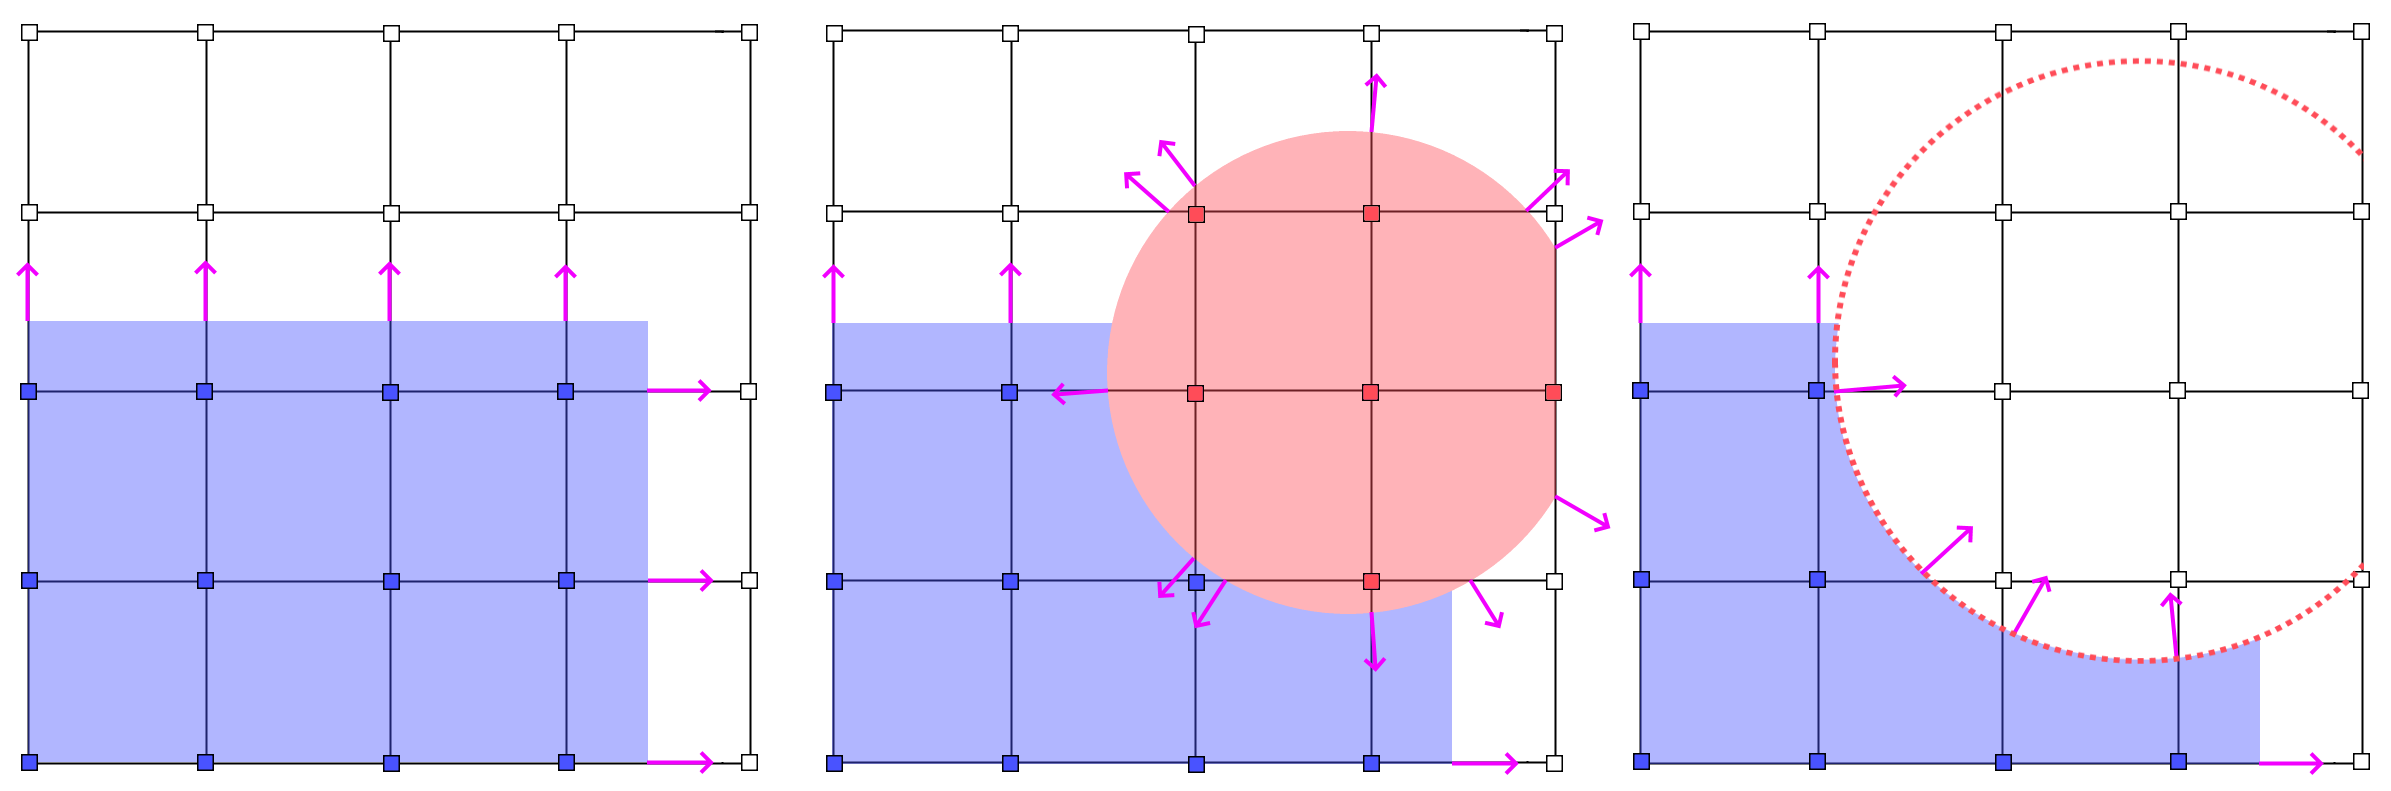
\includegraphics[width=0.8\textwidth]{hermite_data_csg.png}
\caption{CSG operations on a 2D Hermite data voxel grid. From left to right: initial grid, union and difference. Each square and its line segments to the right and above,
including any normals (pink) on them, represent one Hermite data voxel.}
\label{fig:hermite_data_csg}
\end{figure}

The CSG operations that our application uses for the sculpting brushes can be applied using variants of Alg. \ref{alg:hermite_data_csg}. 

\begin{algorithm}[H]
\small
\caption{\textbf{Union.} \textit{Applies a CSG union to a voxel grid. \textsc{FindIntersection} finds the intersection of a primitive with the specified edge
and returns an intersection object. $intersection.distance$ is the distance between the intersection and a voxel or $edge.voxels[0]$, and $intersection.normal$ is the 
surface normal vector at the intersection.}}\label{alg:hermite_data_csg}
\begin{algorithmic}[1]
\Procedure{Union}{VoxelGrid $grid$, CSGPrimitive $primitive$}
	\ForAll{$v \in grid.voxels$}
			\If{$v$ is inside $primitive$}
				\State $v.inside \gets true$
				\State $v.material \gets primitive.material$
			\Else
				\State $v.inside \gets false$
			\EndIf
	\EndFor
	\ForAll{$e \in grid.edges$}
		\If{$e.voxels[0].inside \neq e.voxels[1].inside$}
			\State $intersection \gets$ \Call{FindIntersection}{$e, primitive$}
			\If{$e.voxels[0].inside \land intersection.distance \geq e.voxels[0].intersections[e.axis]$}
				\State $e.voxels[0].intersections[e.axis] \gets intersection.distance$
				\State $e.voxels[0].normals[e.axis] \gets intersection.normal$
			\ElsIf{$e.voxels[1].inside \land intersection.distance \leq e.voxels[0].intersections[e.axis]$}
				\State $e.voxels[0].intersections[e.axis] \gets intersection.distance$
				\State $e.voxels[0].normals[e.axis] \gets intersection.normal$
			\EndIf
		\EndIf
	\EndFor
\EndProcedure
\end{algorithmic}
\end{algorithm}

First, the algorithm for a CSG union operation tags all voxels of the voxel grid that are inside the CSG primitive. Then it iterates over all edges of the voxel grid and checks if the two voxels
that form the edge have a different $inside$ state. If that is the case then the edge must intersect with the primitive's surface and the exact intersection is found
using \textsc{FindIntersection}. The algorithm then checks if any already existing intersections can and must be replaced by comparing their values. For multi-material voxel volumes some additional checks are required, mostly so that intersections are placed correctly at
solid to solid material transitions. In addition to that, our implementation also gives each CSG primitive an axis aligned bounding box, such that only those voxels and edges inside the bounding box need to be checked.\\
With some minor adjustments, namely swapping the $\geq$ and $\leq$, inverting the normals and changing the material assignment at the top to set to empty voxels, the algorithm for the CSG difference operation is obtained. \par

In Section \ref{sec:signed_distance_functions} it was already mentioned that SDF's are well suited for CSG primitives.
The reason for this is that they are versatile and checking whether a voxel lies inside the SDF or finding
line to surface intersection points is simple. Checking whether a voxel is inside the SDF is a simple as checking whether the value of the SDF evaluated at said voxel is negative.
Finding intersection points (\textsc{FindIntersection}) on an edge is done by running a binary search on the edge, starting with the edge start- and endpoints and repeatedly moving them closer together.
The binary search runs as long as the sign at the start- and endpoints are different, or until the value returned by the SDF for either start- or endpoint is within a certain threshold from zero. Both the start- and endpoints will thus converge towards the position where the SDF evaluates to zero, i.e. the SDF's surface.\\

\begin{figure}
\centering
\captionsetup{width=0.8\textwidth}
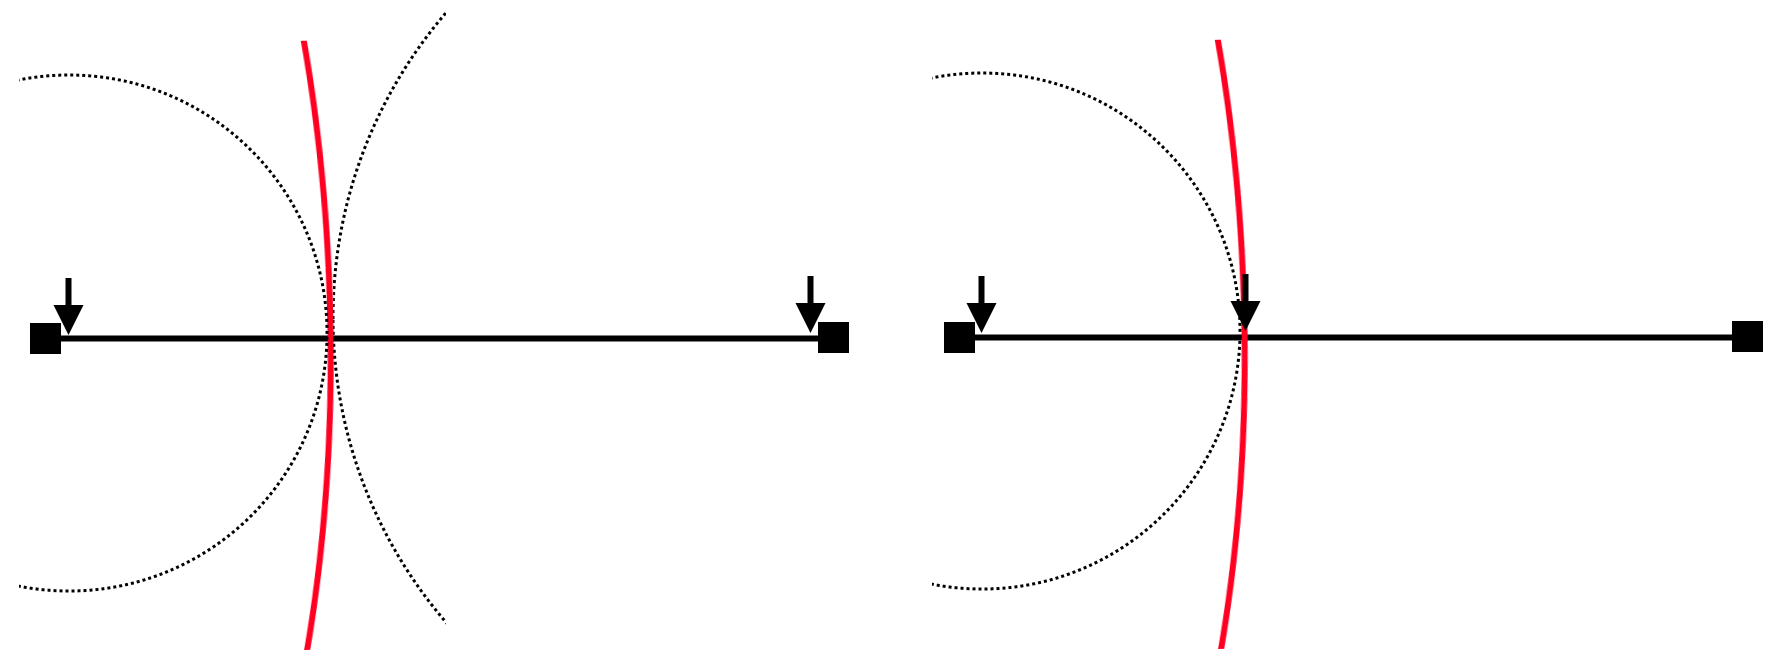
\includegraphics[width=0.5\textwidth]{adaptive_binary_search.png}
\caption{Adaptive binary search. Red circle: SDF's surface, Arrows: start- \& endpoint, Black circles: circles with radius of SDF's value at start- or endpoint. The adaptive binary search
finds the zero point from the initial state (left) after just one iteration (right).}
\label{fig:adaptive_binary_search}
\end{figure}

This binary search can be optimized by using the values returned by the SDF for each iteration. Those values are a lower bound of the distance the start- or endpoint can be moved without accidentally crossing the SDF's surface. Using this fact the adaptive binary search can often make larger and more precise steps than a blind binary search. Consider a nearly linear surface perpendicular to the edge, like in Fig. \ref{fig:adaptive_binary_search}: the adaptive binary search will find the exact zero point after just one iteration because the two values returned by the SDF are the exact distances between the start- and endpoints and the surface. This may not always work for inexact SDF approximations since the returned values may not be actual lower bounds, hence the algorithm should still be able to use the regular binary search method as fallback for robustness.

\subsection{Rendering}
\label{sec:voxel_rendering}
%Vertex colors encode material (RGB, A=texture id), texture array, triplanar texturing shader

\begin{figure}
\centering
\captionsetup{width=0.8\textwidth}
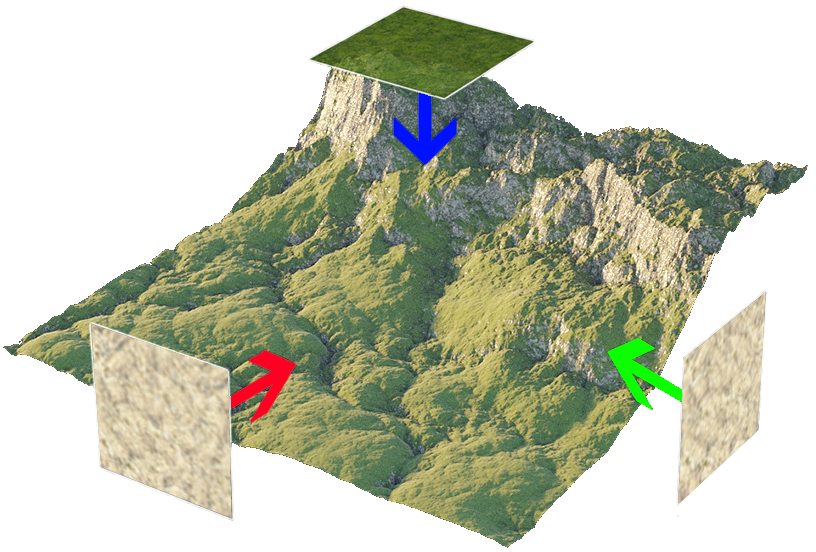
\includegraphics[width=0.4\textwidth]{triplanar_texture_mapping.png}
\caption{Tri-planar texture mapping of a mesh. Note how the hillsides of the terrain are rocky and the top is grassy.
Adapted from \url{https://corona-renderer.com/blog/wp-content/uploads/2017/04/Triplanar_01.jpg}}
\label{fig:triplanar_texture_mapping}
\end{figure}

The voxel polygonizer already does most of the heavy lifting for the voxel rendering. Once the voxel polygonizer has converted the voxels into a triangle mesh the rendering is done using the typical mesh rasterization techniques, provided by Unity, and shaders. Shaders are GPU programs that determine how objects in the scene are rendered to the screen, e.g. by computing lighting or adding special effects. The voxel materials and their colors are packed into the 32 bit RGBA color attachment of the mesh vertices. The first three components, RGB, are used to store the voxel color, the fourth component A for the voxel material ID.\\
Since our voxel meshes are not UV mapped, i.e. they do not contain information about where the textures should be sampled, we have resorted to a tri-planar texture mapping shader to texture them. These kinds of shaders use the position of a mesh's pixels to determine where to sample a texture, without the need of any explicit UV mapping. In order to achieve a realistic looking texture
mapping the tri-planar texture mapping shader projects an infinitely repeating texture from the X, Y and Z axes onto the mesh
like depicted in Fig. \ref{fig:triplanar_texture_mapping}. The weight, i.e. how visible it is, of each texture projection is determined by the mesh's normals. For example the more a normal points along the X axis, the stronger the X axis texture projection is weighted, and the less the other two. The result of this is a mesh
that is usually textured nicely on all sides. In certain situations, especially when the weights of two texture projections are similar, e.g. for $45^{\circ}$ diagonal parts of the mesh with respect to axes, there can be unnatural overlapping of two texture projections. This however is only a problem for textures with obvious structures, e.g. bricks, as opposed to natural or noisy textures like dirt or grass. To support multiple textures we store all voxel material textures in a single texture array on the GPU. The tri-planar texture mapping shader can then select the appropriate texture to sample from for each vertex by using the vertex' voxel material ID, stored in the alpha component, to index into the texture array.

\subsection{Voxelizer}
\label{sec:voxelizer}
% Purpose, explain method used for voxelization (assigning triangles to bins, patching holes, etc.), use of job system

The precursor of our application already had an implementation of a voxelizer, however throughout the development of this thesis
the voxelizer was rewritten to scale better with high triangle counts.\\
The implementation of a basic voxelizer is described in Alg. \ref{alg:voxelize}. This algorithm however will only work properly
for meshes without holes.


\begin{algorithm}[H]
\caption{\textbf{Voxelize.} \textit{Voxelizes the given mesh into the voxel grid. \textsc{FillSection} fills the voxel grid along and inside the given section with the given material and also sets the voxel Hermite data at the section's start and end points.}}\label{alg:voxelize}
\begin{algorithmic}[1]
\Procedure{Voxelize}{VoxelGrid $grid$, Mesh $mesh$, Material $material$}
	\ForAll{$axis \in \{X,Y,Z\}$}
		\ForAll{$voxel \in grid.sideVoxels[axis]$}
			\ForAll{$section \in $ \Call{FindSections}{$axis, voxel.position ,mesh$}}
				\State \Call{$FillSection$}{$grid, section, material$} 
			\EndFor
		\EndFor
	\EndFor
\EndProcedure
\end{algorithmic}
\end{algorithm}

\begin{algorithm}[H]
\caption{\textbf{FindSections.} \textit{Finds all intersections of a line with the mesh and then returns all sections that are between an ingoing and outgoing intersection, i.e. inside the mesh.}}\label{alg:find_sections}
\begin{algorithmic}[1]
\Procedure{FindSections}{Axis $axis$, Position $position$, Mesh $mesh$}
	\State $line \gets$ \Call{CreateLine}{$position, position + axis * gridSize$}
	\State $intersections \gets \varnothing$
	\ForAll{$triangle \in mesh$}
		\State $intersections \gets intersections$ $\cup$ \Call{FindIntersection}{$line, triangle$}
	\EndFor
	\State \Call{Sort}{$intersections$}
	\State $sections \gets \varnothing$
	\State $previous \gets \varnothing$
	\State $inside \gets false$
	\ForAll{$intersection \in intersections$}
		\If{$\neg inside \land previous \neq \varnothing$}
			\State $sections \gets sections$ $\cup$ \Call{CreateSection}{$previous,intersection$}
		\EndIf
		\State $previous \gets intersection$
		\State $inside \gets \neg inside$
	\EndFor
	\State \textbf{return} $sections$
\EndProcedure
\end{algorithmic}
\end{algorithm}

Essentially the algorithm checks the grid lines perpendicular to the +X, +Y and +Z faces of the voxel grid for intersections
with the mesh. Doing this for all the three grid faces will ensure that no triangles or voxels to be filled are missed.
The found intersections are then sorted from minimum distance from grid face to maximum distance. When iterating over these
sorted intersections the algorithm alternates between inside the mesh and outside the mesh, since for each incoming intersection
the next intersection must be an outgoing intersection. All voxels inside such a pair of ingoing and outgoing intersections are
then filled with a chosen material. For the first and last voxel in such a section the algorithm also needs to set the Hermite data, i.e. the voxel intersection values and normals.\\
We have found that in practice some triangles seem to be missed during the intersection checks due to floating point precision errors. To address this problem our implementation performs a post-processing
hole patching algorithm that checks for missing normals in the voxel Hermite data and then obtains them by sampling from the closest
triangle to the hole's position.\\
Note that the complexity of the algorithm, disregarding \textsc{FillSection}, is $O(N^2 * K)$ where $N$ is the voxel grid
size and $K$ the triangle count of the mesh, since for each side voxel touching one of the grid's +X, +Y or +Z faces, of which there are $3*N^2$ in total, the algorithm needs to check all triangles. For large $N$ and $K$ this poses a problem. Hence as improvement our new
algorithm first runs Alg. \ref{alg:assign_triangles}.

\begin{algorithm}[H]
\caption{\textbf{AssignTriangles.} \textit{Projects the AABB's of all triangles onto all three voxel grid faces and then
assigns the triangles to the bin of the according face and position.}}\label{alg:assign_triangles}
\begin{algorithmic}[1]
\Procedure{AssignTriangles}{Bins $bins$, Mesh $mesh$}
	\ForAll{$axis \in \{X,Y,Z\}$}
		\ForAll{$triangle \in mesh$}
			\State $box \gets$ \Call{CreateAABB}{$triangle$}
			\State $area \gets$ \Call{ProjectOnGridFace}{$axis,box$}
			\ForAll{$position \in area$}
				\State $bins[axis][position] = bins[axis][position] \cup triangle$
			\EndFor
		\EndFor
	\EndFor
\EndProcedure
\end{algorithmic}
\end{algorithm}

Following that Alg. \ref{alg:find_sections} is then modified to only iterate over the triangles in $bins[axis][position]$.
In practice this provides a good speed improvement, although at the cost of more memory, because Alg. \ref{alg:find_sections} will
only have to check a tiny fraction of all the triangles for each position.\\
In our implementation \textsc{FindSections} runs in parallel for all the voxels touching one grid face since all the voxels along one
of the face's perpendicular grid lines can be written to independently in parallel. This is done three times, once per grid face, because otherwise the algorithm could potentially write to the same voxel multiple times at the same time, causing a write conflict.

\section{VR Sculpting}

The feature that ties all these technologies together is the VR sculpting. It allows the user to freely sculpt arbitrary shapes or figures by using voxels, CSG operations and various brush shapes.

\subsection{SteamVR Plugin}

The implementation of our VR application was realized through the Unity SteamVR Plugin\footnote{\url{https://assetstore.unity.com/packages/tools/integration/steamvr-plugin-32647}}. This Unity plugin offers most of the base functionality required for VR applications, such as setting up the headset and controller tracking and handling controller input. Furthermore it provides some additional scripts that can be added to objects in the scene, for example to allow the player to teleport or to grab and hold objects.\\
Unfortunately certain features of the SteamVR Plugin are currently not yet compatible with Unity's new Universal Render Pipeline\footnote{\url{https://docs.unity3d.com/Packages/com.unity.render-pipelines.universal@8.1/manual/index.html}} (URP) that handles the rendering of scenes. With the introduction of the URP the format of Unity's
shaders has changed. Some of these shaders, most notably the highlight when grabbing an object, were required for our application and thus had to be partially rewritten to work in the new URP.

\subsection{Sculpting Functionality}
%How sculpting is implemented, VRSculpting controller, etc.

The sculpting functionality is split into several scripts and components. The following list goes through the most important components for the sculpting functionality. The term "script" refers to a C\# class extending \textsc{MonoBehaviour} in the Unity project and "component" refers to a script that has been instantiated and added to an object. \textsc{MonoBehaviour}'s are scripts that can be attached to objects in the scene.

\subparagraph{Voxel Sculpture}
The voxel sculpture/terrain functionality is provided by the \textsc{DefaultVoxelWorldContainer} script and can be added as a component to an empty object. This object is then capable of storing and rendering voxels and can be modified through the \textsc{ApplySdf} method in \textsc{DefaultVoxelWorldContainer.Instance}.

\subparagraph{Texture Array}
As mentioned in Section \ref{sec:voxel_rendering} our application uses a texture array to store all the voxel material textures on the GPU for rendering. This texture array is created by the \textsc{VoxelTerrainTextures} script which is to be added to the same object that contains the \textsc{DefaultVoxelWorldContainer} component. On start of the application it reads all the textures that have been added to the \textsc{VoxelTerrainTextures} component's textures array into a texture array on the GPU and then assigns it to the "\_TextureArray" attribute of the object's material such that the tri-planar texturing shader can access it.

\subparagraph{Brush Type Renderers}
All regular brush types need some way to be rendered as a preview. For each brush type a unique \textsc{ISdfRenderer} instance is responsible for rendering. The regular way to obtain such a renderer is to create a \textsc{MeshSdfRenderer} object which extends \textsc{ISdfRenderer} and handles all the rendering when given a mesh. Such an object is created in Unity's context menu under "Create $\rightarrow$ ScriptableObject $\rightarrow$ MeshSdfRenderer". Once created a mesh and material must be assigned to the object. Optionally an offset and scale can be specified. For advanced brushes one may create a custom renderer by extending \textsc{ISdfRenderer}.\\
These renderers by themselves aren't useful yet. They need to be registered to the "Static Renderers" menu of the \textsc{SdfShapeRenderHandler} component on the player object.

\subparagraph{Custom Brush}
The main functionality of the custom brushes is contained in the \textsc{DefaultCustomBrushContainer} script which is found on a seperate object. It mostly handles creating the SDF from a list of custom brush primitives. In order to be able to render the custom brush is in the \textsc{DefaultCustomBrushSdfRenderer} script which is usually on the same object as the \textsc{DefaultCustomBrushContainer}. The custom brush can be edited by changing the \textsc{DefaultCustomBrushContainer.Instance.Primitives} list which contains the current custom brush primitives.

\subparagraph{Undo/Redo}
The undo/redo functionality is handled by the \textsc{DefaultVoxelEditManagerContainer} script. It exposes an \textsc{Undo} and \textsc{Redo} method in \textsc{DefaultVoxelEditManagerContainer.Instance}. In order to store edits \textsc{DefaultVoxelEditManagerContainer.Instance.Consumer()} must be passed to \textsc{ApplySdf}. Brush strokes are counted as a single edit. Each edit stores a snapshot of the previous state of the chunks it affects so the edit can be undone by replacing the chunk data with the snapshots.

\subparagraph{VR Interaction}
The core of the application that ties everything together is the \textsc{VRSculpting} script found on the player object. It handles all the interactions between the sculpture, voxels, brushes, queries, UI's and so on.

\subparagraph{Cineast API}
Communication with Cineast is handled through the \textsc{UnityCineastApi} script. A query is started by calling \textsc{StartQuery} with the model data and once the results are back the \textsc{UnityCineastApi} relays them to the \textsc{QueryResultSpawner} which handles displaying the results.\\


\subsection{Sculpting Tools}
%General overview of capabilities and functionality, UIs, SteamVR Plugin, etc.

Our VR sculpting application provides several tools to enable the user to sculpt.

\subparagraph{Controller Hints}

\begin{figure}
\centering
\captionsetup{width=0.8\textwidth}
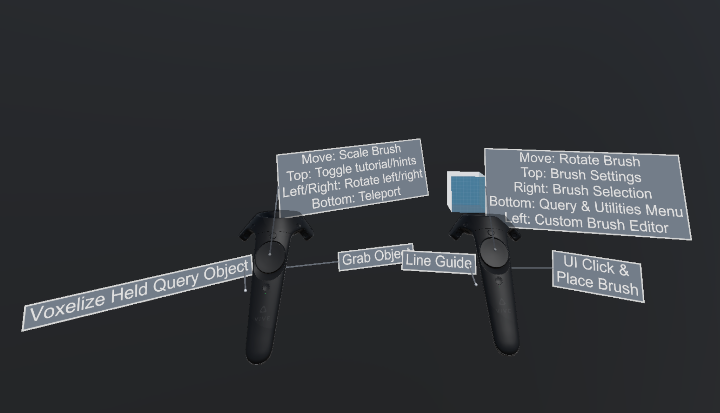
\includegraphics[width=0.75\textwidth]{controller_hints.png}
\caption{Controller hints}
\label{fig:controller_hints}
\end{figure}

The controller hints portrayed in Fig. \ref{fig:controller_hints} help the user become familiar with the VR sculpting application. They are always shown when the application is started but can then be toggled on or off by pressing a button on the controller.\\
This controller hints functionality is provided as a script in the SteamVR plugin package, however we modified it to make it possible to specify on which side to place the hints. Before this modification all hints were always placed on the right side of the controller, causing some of them to overlap.

\subparagraph{Brush}

\begin{figure}
\centering
\captionsetup{width=0.8\textwidth}
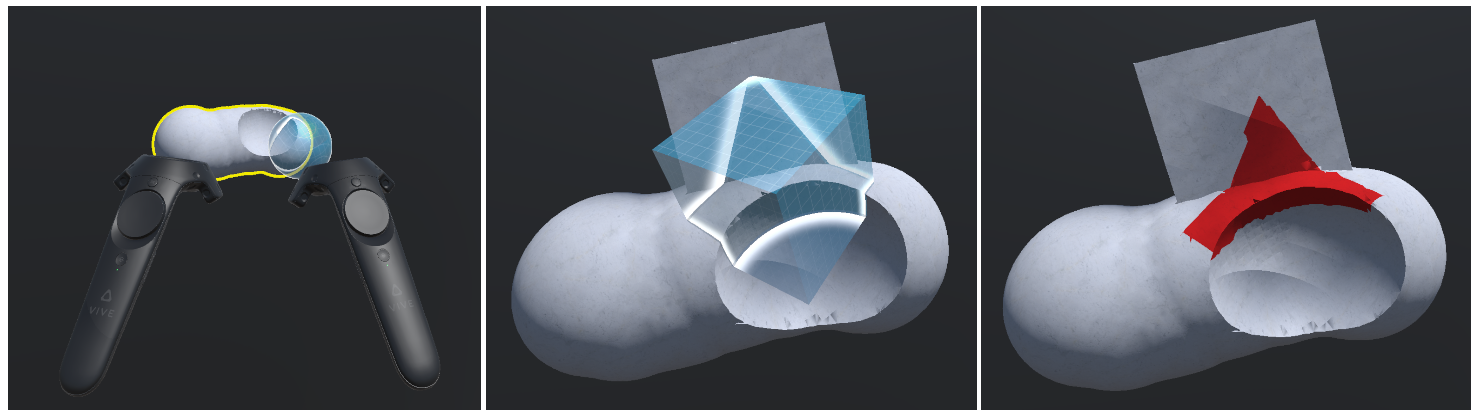
\includegraphics[width=0.75\textwidth]{editing_showcase.png}
\caption{Illustration of the sculpting process. Left: modifying a sculpture. Middle: brush preview with intersection highlight. Right: after applying brush in replace mode with a red material.}
\label{fig:editing_showcase}
\end{figure}

The most important tool available to the user is the brush. It is attached to the right controller as depicted in Fig. \ref{fig:editing_showcase} and displayed as a translucent preview of the brush's shape. Using a custom shader this brush preview shows the intersection between the brush and the sculpture. This feature has turned out to be an important addition, because without it it's quite difficult to tell where the brush intersects with the sculpture despite the stereoscopic display of the VR headset.\\
By holding the brush button, which is by default the index finger trigger on the right controller, the user can drag the brush and continuously apply a brush stroke so long performance allows.\\
The brush size can be changed by swiping up or down on the trackpad of the left controller. Similarly the brush can be rotated by swiping any direction on the trackpad of the right controller. Rotating the brush however takes some practice because the trackpad only provides two degrees of freedom whereas there are three rotation axes for the brush.\\
Currently our application provides five brush types: cube, sphere, pyramid, cylinder and custom. These brush types are defined from SDF's, thus it is easy to add new brush types. Our VR application provides some Unity editor interfaces to enable a developer to easily add such new brushes to the application.

\subparagraph{Brush Settings}

\begin{figure}[!htb]
\minipage{0.49\textwidth}
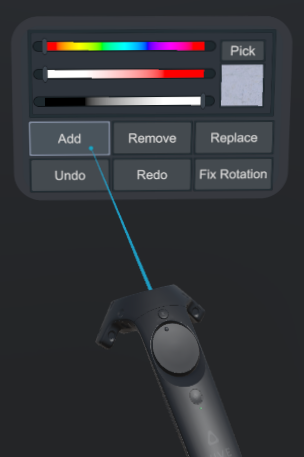
\includegraphics[width=\linewidth]{gui_brush_properties.png}
\caption{Brush properties menu}
\label{fig:gui_brush_properties}
\endminipage\hfill
\minipage{0.49\textwidth}
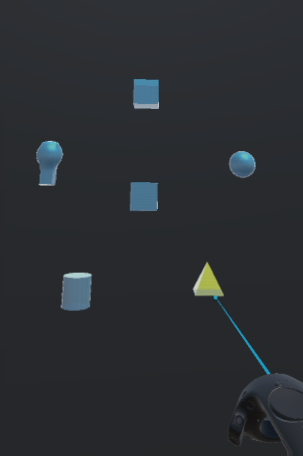
\includegraphics[width=\linewidth]{gui_brush_select.png}
\caption{Brush selection menu}
\label{fig:gui_brush_select}
\endminipage\hfill
\end{figure}

These brushes are only useful if the user can adjust the brush and its behaviour to their liking. Fig. \ref{fig:gui_brush_properties} shows the brush properties menu which contains all the brush settings that can be changed.\\
The user can change the CSG operation using the "Add", "Remove" and "Replace" buttons. During development we decided to replace the CSG terminology "Union" and "Difference" with the more common words "Add" and "Remove" to make it more intuitive for users that do not know anything about CSG.\\
The three sliders are used to change the color of the brush material. We decided to use this three slider style Hue/Saturation/Value (HSV) color selection because it immediately presents the user with a large spectrum of colors that can be finely adjusted with the saturation and value, i.e. brightness, sliders. The color preview box on the right shows how the brush material will look with the color applied. Once the sculpture has been colored with a certain color the user can always reselect that color by pressing the "Pick" button and then clicking on the spot of the sculpture with the desired color.\\
The brush material texture is changed by clicking on the color preview box which opens a submenu and then clicking on another texture in that submenu.\\
By default, the brush is fully attached to the right controller which means that it also rotates with the controller. If that is not desired then the user can toggle the
"Fix Rotation" button. This disables the automatic rotation of the brush with the controller making it easier to for example to create straight lines with the brush.\\
If the user has made a mistake it can be undone by clicking the "Undo" button. Currently up to ten edits can be undone. Edits that have been undone can be redone by clicking the "Redo" button, however only if the user has not edited the sculpture again since the undo.\\
The brush selection menu in Fig. \ref{fig:gui_brush_select} lets the user select different brushes. It is arranged as a radial menu centered in front of the user's right controller. Like this the user quickly and conveniently select other brush types without having to move the controller much.

\subparagraph{Custom Brushes}

\begin{figure}
\centering
\captionsetup{width=0.8\textwidth}
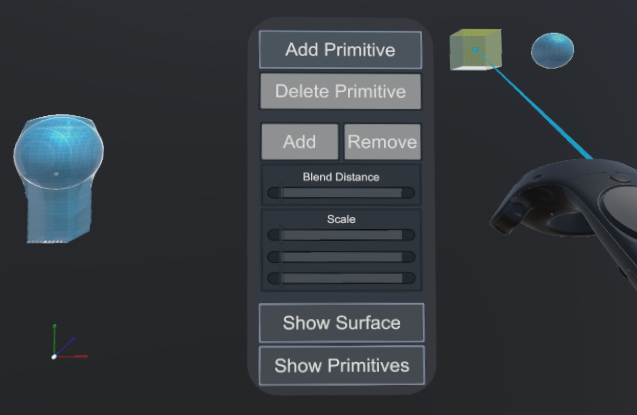
\includegraphics[width=0.75\textwidth]{gui_custom_brush.png}
\caption{The custom brush editing menu used to create custom brush shapes. A custom brush shape composed of a sphere and scaled cube is shown on the left side. The shapes are blended together smoothly resulting in a brush shape that looks like a cuboid that bulges out at the top.}
\label{fig:gui_custom_brush}
\end{figure}

Our application currently only supports hard boolean CSG, meaning that union and difference operations often lead to sharp edges and corners. This is not always desirable, especially when the user wants to sculpt organic and
smooth shapes. One solution to address this would be to implement a smoothing brush that smooths out sharp edges, e.g. by averaging the positions of the surface vertices and adjusting the normals. However doing this is not trivial
because the surface vertices are constructed from the underlying voxels, hence the smoothing would instead have to happen in the voxel data instead. This also leads to several edge cases like when a voxel Hermite data intersection is moved
from one voxel to another care must be taken to also adjust the intersections on the other voxel edges such that it doesn't produce a hole in the mesh. The multi-material voxels also pose a problem because the smoothing brush should
not disturb or even destroy the material transitions.\\
To avoid all these troubles we have conceived a proof of concept custom brush that can be shaped by the application's user. As discussed previously SDF's can be smoothly blended together using the smooth minimum and maximum operators.
Our custom brushes take advantage of that and enable the user to smoothly blend two or more SDF primitives together to create a brush shape. Currently our application supports combining cube and sphere primitives together, but new
primitives can be added easily in almost the same way as it is done for the regular brushes. In addition to that each SDF primitive can be scaled on all three axes independently.\\
These custom brushes have several use cases: they can be used to create a single primitive shape that can be scaled, e.g. creating an ellipsoid from a sphere primitive, or it can be used to create more complex shapes, such as e.g.
a rounded disc by combining one sphere primitive and smoothly subtracting two cube primitives from the top and bottom of the sphere.

\subsection{VR User Interface System}

\begin{figure}
\centering
\captionsetup{width=0.8\textwidth}
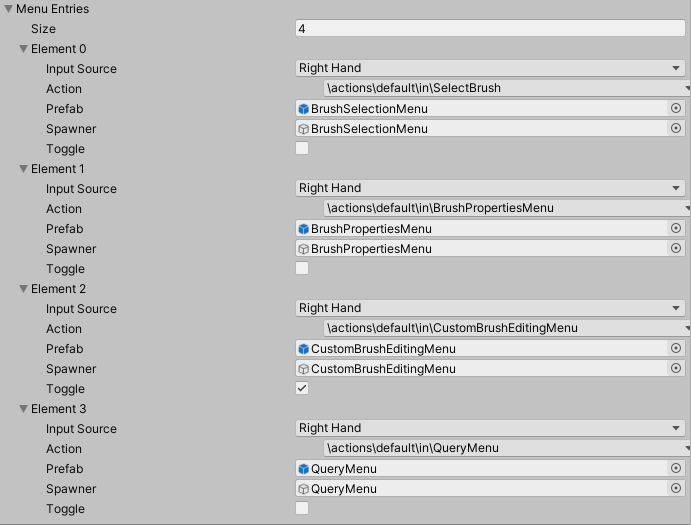
\includegraphics[width=0.75\textwidth]{adding_menus.png}
\caption{Menu entries section in the \textsc{VRSculpting} component where developers can register new UI's.}
\label{fig:adding_menus}
\end{figure}

We have implemented a flexible system for VR user interfaces (UI) in Unity. Most of our menus are similar to what you would expect in a regular non-VR application. The reason for this is that most users will already be familiar with the typical window based UI's found in modern operating systems. Furthermore, such window based UI's can densely pack information and functionality while remaining organized and hierarchical, e.g., by using grouping background elements such as the color settings group in Fig. \ref{fig:gui_brush_properties} to group contextually similar components together.\\
The UI's are controlled by the VR controller, which has a pointer and cursor attached to it. Since our application uses the SteamVR Plugin, we have designed our pointer and cursor to be similar to that of the SteamVR menu to maintain consistency. UI components can be interacted with by pressing the interaction button on the VR controllers which by default is bound to the index finger trigger on the right controller.\\
New UI's can easily be created by creating a new empty object and then adding Unity's \textsc{Canvas} component. This turns the object into a UI canvas and the developer can add UI elements to the viewport specified in the \textsc{Canvas} component. Any UI element already available in Unity should work in VR out of the box. This is made possible by our \textsc{VRPointerInputModule} script, which extends Unity's \textsc{BaseInputModule} and thus replaces Unity's default keyboard and mouse based input controller with our VR pointer input controller. Once a new UI is finished it is converted into a Unity prefab and then registered in order to become usable by the user. This is done in the Unity editor in the \textsc{VRSculpting} component on the player object under the "Menu Entries" section. Within this section, depicted in Fig. \ref{fig:adding_menus}, the developer can add a new entry, then set the prefab field to point to the UI prefab, set which controller button should open the UI, whether it is toggled and where it should appear when opened.

\subsection{Similarity Query}

\begin{figure}
\centering
\captionsetup{width=0.8\textwidth}
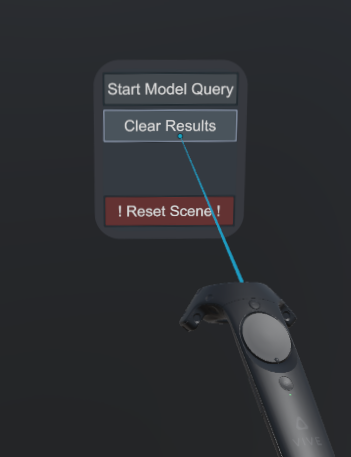
\includegraphics[width=0.3\textwidth]{gui_query.png}
\caption{Query menu with buttons to start a query, clear query results and to reset the entire scene.}
\label{fig:gui_query}
\end{figure}

Similarity queries are executed by clicking the "Start Model Query" button in the query menu shown in Fig. \ref{fig:gui_query}. The application then converts the current sculpture into a single mesh and sends it to Cineast to be processed.

%\begin{figure}
%\centering
%\captionsetup{width=0.8\textwidth}
%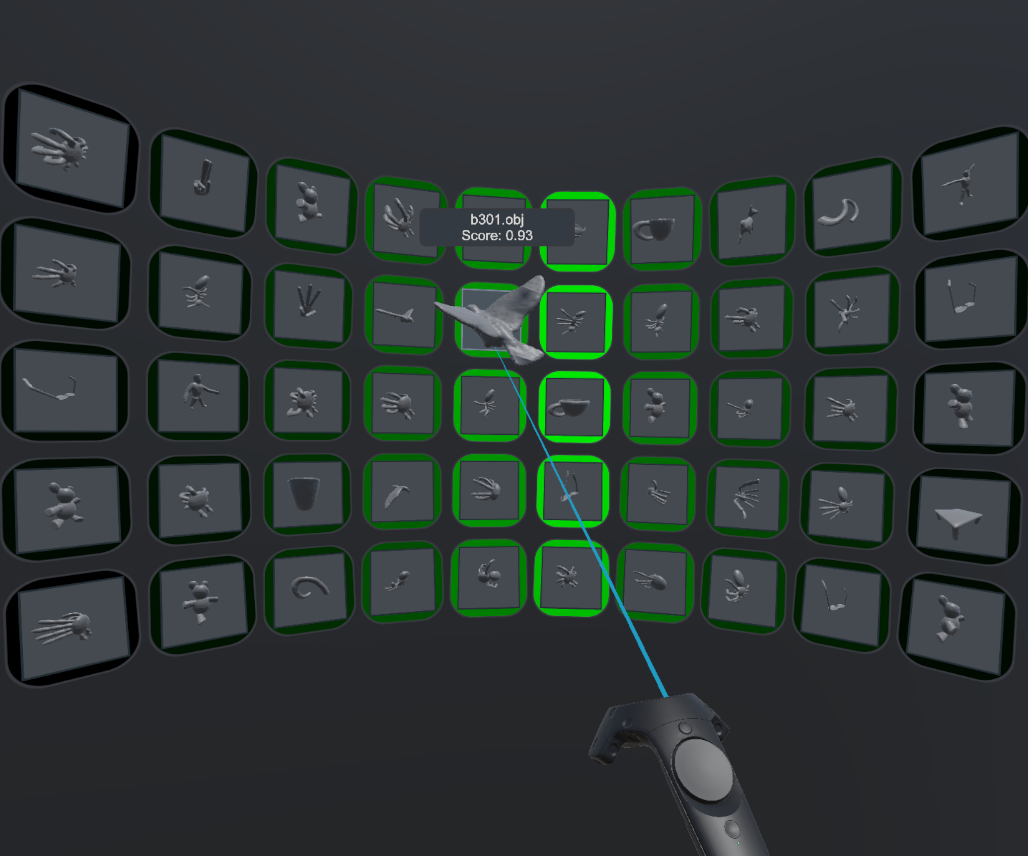
\includegraphics[width=0.75\textwidth]{query_pointing.png}
%\caption{Query results UI showing the results of a similarity query.}
%\label{fig:query_pointing}
%\end{figure}

%\begin{figure}
%\centering
%\captionsetup{width=0.8\textwidth}
%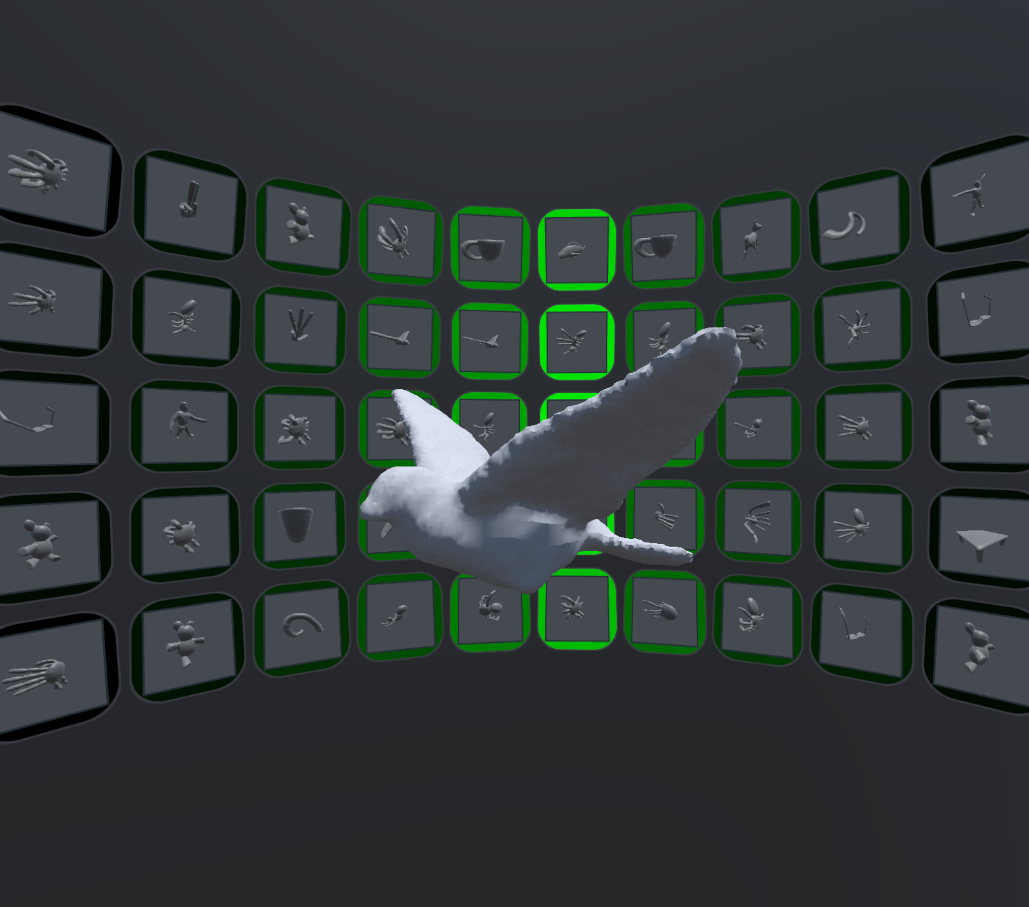
\includegraphics[width=0.75\textwidth]{query_voxelized.png}
%\caption{A voxelized and fully editable model from the query results UI.}
%\label{fig:query_voxelized}
%\end{figure}

\begin{figure}[!htb]
\minipage{0.49\textwidth}
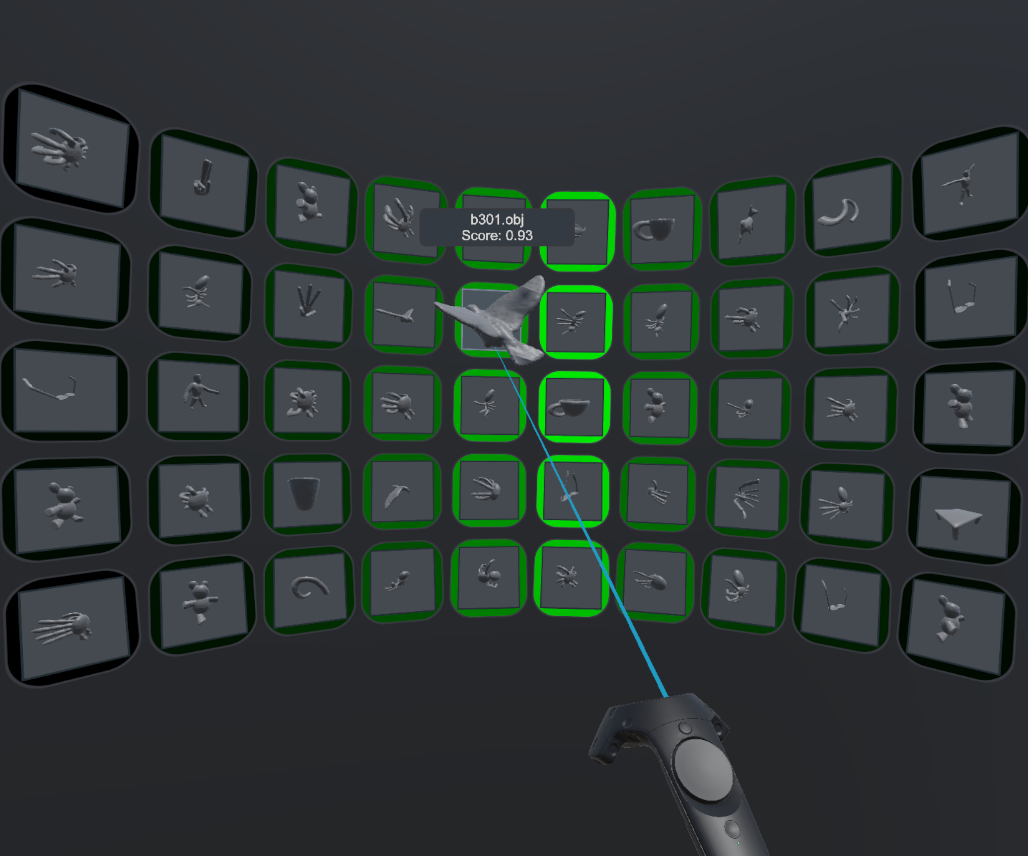
\includegraphics[width=\linewidth]{query_pointing.png}
\caption{Query results UI showing the results of a similarity query.}
\label{fig:query_pointing}
\endminipage\hfill
\minipage{0.49\textwidth}
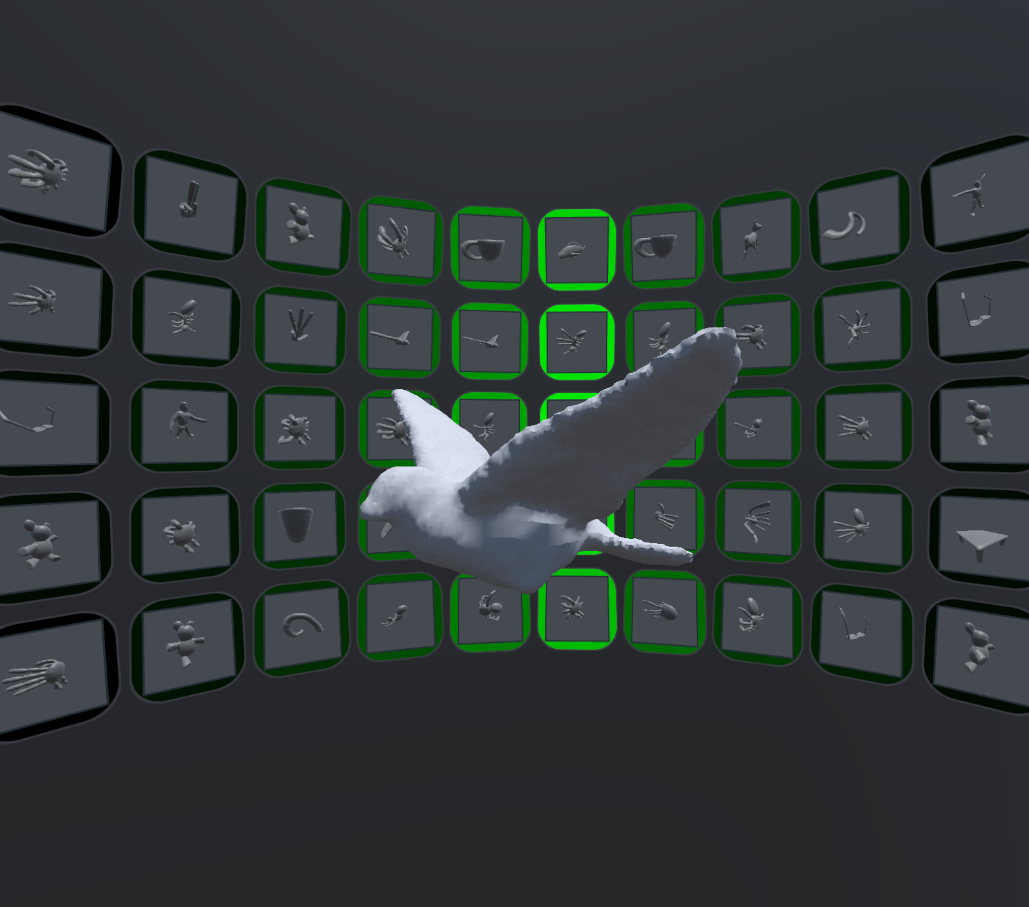
\includegraphics[width=\linewidth]{query_voxelized.png}
\caption{A voxelized and fully editable model from the query results UI.}
\label{fig:query_voxelized}
\endminipage\hfill
\end{figure}

Once the results have arrived back at the VR sculpting application they are displayed in a curved UI centered on the player's head. The intention is to be able to use the entire $360^{\circ}$ available in VR to display as many results as possible. Unfortunately due to performance problems while loading the results in and a networking problem in the API communication this is not yet possible, but certainly achievable in the future.\\
The user can point at query results which makes a 3D model object appear and spin around their Y axis. Additionally this shows their name and the similarity score value on a label above the model. These model objects can be grabbed with the left controller for closer inspection.\\
Fig. \ref{fig:query_pointing} portrays the curved query results UI with the user pointing at a result object. When held in the left controller the 3D model objects can be voxelized, i.e. converted into a voxel sculpture like in Fig. \ref{fig:query_voxelized}. This sculpture is then fully modifiable using the sculpting tools and can be used to create a new query. This allows the user to start with a rough 3D sketch to perform an initial query and then successively refine the query until the user finds the desired object.
\chapter{Evaluation}

\section{Technical Evaluation}
Voxelizer, polygonization, queries, precision vs. recall?, etc.

\section{User Evaluation}

\subsection{Structure}

\subsection{Results}

TBD after evaluation
\chapter{Discussion}

\section{Conclusion}

\section{Lessons learned}

\section{Future work}
%Performance, LODs/Octrees (SVO)/memory use (e.g. run length encoding), meshes as brushes (using voxelizer), saving/loading sculptures \& custom brushes, multiple sculptures at once, splitting sculptures.\\
%More brush features, e.g. selecting a polygon and filling it with material. Line guide could automatically fill between start/end.\\
%Custom brush editor could use mean position of primitives as brush center.\\
%Add way to run exact more like this query without voxelization.

While our VR sculpting application already provides a solid base to work off of there are still many improvements required for it to become a mature sculpting application.

\subsection{Performance}
The main problem currently is the performance of the sculpting and rendering. The sculpture mesh does not use any level of detail (LOD) system or adaptive data structure and as such the resulting meshes have very high triangle counts.
Eventually when a sculpture becomes large enough the framerate will drop below the desired 120Hz for VR. This problem could be addressed by using an adaptive data structure like Octrees to reduce the complexity of the meshes and only keep the details where necessary. This approach has already been tried and discussed in [\todoMissing{Missing ref; DC}].\\
Closely related is also the memory usage of sculptures which could be reduced by using adaptive data structures and compression schemes. A commonly used compression scheme for voxels is Run Length Encoding (RLE), where instead of storing
each voxel in an array the program stores runs of voxels. Each run is described by the length of the run and the single voxel data. In most cases this leads to a good compression because large parts of sculptures are uniform, i.e. contain the same voxel data.

\subsection{Usability}

\subparagraph{Sculpting}
The sculpting module currently misses some features that would increase usability of our application by a lot.\\
Our brushes are based entirely on SDF's and while those are quite flexible a user may instead want to use a mesh as brush shape. The voxelizer module could be used to compute the voxel representation of such a mesh, store it in a seperate voxel grid, and then copy that voxel grid to the sculpture when the brush is being applied.\\
Currently only one sculpture can exist at once. Technically multiple sculptures can exist at once, but our application does not yet offer the interaction functionality yet to select which sculpture the user wants to edit. Furthermore when adding multiple sculptures it would make sense to implement an algorithm that is able to detect when a sculpture has multiple disjoint parts so that they can each be converted into seperate sculptures.\\
One participant of the user evaluation has suggested to add a brush mode where the user selects two or more points to form a line or polygon and the application then automatically fills in that shape. This feature would be very useful to construct more precise shapes.

\subparagraph{Custom Brush Editor}
While the custom brush editor is functional it is not yet useful to create brush shapes with more than three or four primitives. The performance decreases with every primitive added to the brush because whenever a primitive is changed the entire custom brush shape needs to be recomputed. Secondly the editor interface is not yet intuitive and users have found it difficult to edit their custom brushes. One reason for this was the confusion between the "Add/Remove" buttons, which changes the selected primitive's CSG operation, and the "Add/Delete Primitive" buttons, which add or remove a primitive from the custom brush. This could be fixed by using better wording and appropriate icons. Selecting a primitive was also perceived as difficult because it requires the user to point at the center of the primitive with the right controller and then click the trigger, in the same way one would click a button. It would make more sense to change selecting a primitive to be done with the left controller similarly to grabbing an object.

\subparagraph{Saving/Loading}
There is currently no way to persistenly save a sculpture or custom brush. It would make sense for the application to be able to export sculptures or custom brushes into a file on disk so the user can later load them again.

\subparagraph{Queries}
As mentioned before due to some performance issues while loading results and a networking problem the number of results shown in the query results UI is currently limited to 50 results. The networking problem is caused because the C\# Cineast API wrapper sends too many REST requests and the RestSharp\footnote{https://github.com/restsharp/RestSharp} library responsible for sending the requests retains the socket connections open for a while instead of immediately closing them\footnote{https://github.com/restsharp/RestSharp/issues/1322}. This causes the machine to run out of sockets and then refuses to send any further REST requests. The solution would be to use a socket pool and to specify a maximum number of requests that can be in process at once.

\subparagraph{Controls}
It was mentioned several times during the user evaluation that the current control scheme is not optimal. As shown in Fig. \ref{fig:controller_hints} nearly all the controller buttons have been assigned a function, including the difficult to use side grip buttons of the controller. Many participants had trouble finding these side grip buttons and then use them as intended. These problems could be resolved by introducing multiple control schemes or modes that can be switched between while using the application. There could be a mode for just editing the sculpture, including brush controls and the two brush UI's, a mode for just the queries, and so on. This would reduce the amount of buttons required at any one point because the controls are distributed over the different modes.

%% ----------------------------------------------------------------
\thesisappendix
\thesisbib
\begin{appendices}
	\chapter{Appendix}

\section{User Evaluation Questionnaire}

% PDF stuff
\ifx\pdfoutput\undefined
\else
    \pdfpagewidth=210mm
    \pdfpageheight=297mm
\fi

\newif\ifbanner\bannerfalse
\bannerfalse
\advance\oddsidemargin-5mm
\advance\textwidth1cm

\font\manual=manfnt
\def\shared{\noindent\llap{\manual\char'170\kern.15em}}

\def\heading#1{
    \ifhmode\par\fi
    \removelastskip
    \vskip1ex plus 0.5ex minus 0.3 ex%\goodbreak
    \noindent
    \hbox to \hsize{ #1\hfill}
    \smallskip\par\nobreak}


\def\nicefrac#1/#2{\leavevmode%
    \raise.5ex\hbox{\the\scriptfont0 #1}%
    \kern-.1em/\kern-.15em%
    \lower.25ex\hbox{\the\scriptfont0 #2}}

\newdimen\scalewidth
\scalewidth=0.3\hsize 

\def\xboxit#1{\hbox{\lower0.7ex\vbox{\hrule\hbox{\vrule\kern1pt
    \vbox{\kern1pt\hbox{\strut\small #1}\kern1pt}\kern1pt\vrule}\hrule}}}

\def\boxit#1{\hbox{\lower0.7ex\vbox{\hrule\hbox{\vrule\kern1pt
    \vbox{\kern1pt\hbox to 1.4em
    {\small\strut\hfil #1\hfil}\kern1pt}\kern1pt\vrule}\hrule}}}

\def\sboxit{\hbox{\lower0.7ex\vbox{\hrule\hbox{\vrule\kern1pt
    \vbox{\kern1pt\hbox to 1ex
    {\small\strut\hfil}\kern1pt}\kern1pt\vrule}\hrule}}}


\def\fiveboxes#1#2#3#4#5{\hbox to\scalewidth
    {\boxit{#1}\hfil\boxit{#2}\hfil\boxit{#3}\hfil%
     \boxit{#4}\hfil\boxit{#5}}}
\def\manyboxes{\hbox to \scalewidth
    {\sboxit\hfil\sboxit\hfil\sboxit\hfil\sboxit\hfil\sboxit\hfil%
    \sboxit\hfil\sboxit\hfil\sboxit\hfil\sboxit\hfil\sboxit\hfil\sboxit}}


\def\boxes{\fiveboxes{}{}{}{}{}\ignorespaces}

\def\void{\boxit{}}

\def\xscale#1#2{%
    \setbox0=\hbox{\boxes}%
    \setbox1=\hbox to \wd0{\small\strut\hfill #2 $\to$}%
    \setbox2=\hbox to \wd0{\small\strut $\gets$ #1 \hfill}%
    \vbox{\vbox to 0pt{\vss\box1\box2\kern2pt}\vbox{\box0}}}

\def\scale#1#2{%
    \setbox0=\hbox{\boxes}%
    \setbox1=\hbox to \wd0{\small\strut\hfill #2 $\to$}%
    \setbox2=\hbox to \wd0{\small\strut $\gets$ #1 \hfill}%
    \vbox{\medskip\box1\box2\kern2pt\box0}}

\def\xshortscale#1#2{%
    \setbox0=\hbox{\boxes}%
    \setbox1=\hbox to \wd0{\small\strut $\gets$ #1 \hfill #2 $\to$}%
    \vbox{\vbox to 0pt{\vss\box1\kern2pt}\vbox{\box0}}}

\def\shortscale#1#2{%
    \setbox0=\hbox{\boxes}%
    \setbox1=\hbox to \wd0{\small\strut $\gets$ #1 \hfill #2 $\to$}%
    \vbox{\medskip\box1\kern2pt\box0}}

\def\agree{\scale{strongly disagree}{agree completely}}
\def\xagree{\xscale{strongly disagree}{agree completely}}
\def\xquality{\xshortscale{poor}{outstanding}}
\def\quality{\shortscale{poor}{outstanding}}

\def\longquality{%
    \setbox0=\hbox{\manyboxes}%
    \setbox1=\hbox to \wd0{\small\strut $\gets$ poor \hfill outstanding $\to$}%
    \vbox{\vbox to 0pt{\vss\box1\kern2pt}\vbox{\box0}}}

\def\linscale{%
    \def\tick{\vrule height 5pt\relax}%
    \vbox{\hbox to \scalewidth{\tick\hfil\tick\hfil\tick\hfil\tick}\hrule}}

\def\question#1\par#2\par{\hbox to \hsize
    {\vbox{\hsize=0.72\hsize #1\dotfill}\quad#2\hfil}\medskip\goodbreak}

\def\freequestion#1\par{#1\par\nobreak
    \begingroup\nobreak
    \advance\leftskip by 2pc
    \hrule width 0pt height 1.7\baselineskip\hrulefill
    \hrule width 0pt height 1.7\baselineskip\hrulefill
    \par
    \medskip
    \endgroup
    }
		
\def\longfreequestion#1\par{#1\par\nobreak
    \begingroup\nobreak
    \advance\leftskip by 2pc
    \hrule width 0pt height 1.7\baselineskip\hrulefill
    \hrule width 0pt height 1.7\baselineskip\hrulefill
    \hrule width 0pt height 1.7\baselineskip\hrulefill
    \hrule width 0pt height 1.7\baselineskip\hrulefill
    \hrule width 0pt height 1.7\baselineskip\hrulefill
    \hrule width 0pt height 1.7\baselineskip\hrulefill
    \par
    \medskip
    \endgroup
    }

\parindent0pt
\parskip5pt plus 0.2 ex minus 0.1ex


\def\<#1>{\textsc{#1}}
\parindent0pt
\parskip5pt plus 0.2 ex minus 0.1ex

%\begin{document} 

The purpose of this user evaluation is to gather insight and feedback about the current implementation
of the sculpting and querying functionality and the impression it has on users. The results will be
helpful in identifying shortcomings and to improve the user experience.\\ \hfill
If at any point you feel unwell or nauseous while using the VR headset please let me know. That can be a common reaction when not used
to VR or when the program is not responsive enough.\\ \hfill
Each time before moving on a next task please press the X \todoMissing{Which button?} button to reset the scene.


\newcounter{questionnumber}

\hfill \break
\heading{\textbf{Background}}

1: not at all, 2: slighty, 3: moderately, 4: very, 5: extremely \newline


\fbox{\begin{minipage}{1.05\linewidth}
\begin{minipage}{0.95\linewidth}
\question \stepcounter{questionnumber} \textbf{\arabic{questionnumber}.} How experienced are you with Virtual Reality? \par \fiveboxes{\color{gray}1}{\color{gray}2}{\color{gray}3}{\color{gray}4}{\color{gray}5} \par
\end{minipage}
\end{minipage}}


\fbox{\begin{minipage}{1.05\linewidth}
\begin{minipage}{0.95\linewidth}
\question \stepcounter{questionnumber} \textbf{\arabic{questionnumber}.} How experienced are you with 3D sculpting applications? \par \fiveboxes{\color{gray}1}{\color{gray}2}{\color{gray}3}{\color{gray}4}{\color{gray}5} \par
\end{minipage}
\end{minipage}}

\hfill \break
\heading{\textbf{Sculpting}}

1: very easy, 2: easy, 3: neutral, 4: difficult, 5: very difficult \newline

\fbox{\begin{minipage}{1.05\linewidth}
\begin{minipage}{0.95\linewidth}
\question \stepcounter{questionnumber} \textbf{\arabic{questionnumber}.}
Read the controller hints to become familiar with VR and the control scheme. Disable the controller hints once you're ready.\\ \hfill
Time limit: 5min.
\par \fiveboxes{\color{gray}1}{\color{gray}2}{\color{gray}3}{\color{gray}4}{\color{gray}5}

\freequestion Feedback: \par
\end{minipage}
\end{minipage}}


\fbox{\begin{minipage}{1.05\linewidth}
\begin{minipage}{0.95\linewidth}
\question \stepcounter{questionnumber} \textbf{\arabic{questionnumber}.}
Select the sphere brush and place it the world to create a shape or simple sculpture using the 'Add' mode.\\ \hfill
Time limit: 3min.
\par \fiveboxes{\color{gray}1}{\color{gray}2}{\color{gray}3}{\color{gray}4}{\color{gray}5}

\freequestion Feedback: \par
\end{minipage}
\end{minipage}}


\fbox{\begin{minipage}{1.05\linewidth}
\begin{minipage}{0.95\linewidth}
\question \stepcounter{questionnumber} \textbf{\arabic{questionnumber}.}
Select a brush and create a shape, then select another brush and remove a piece of your sculpture with it using the 'Remove' mode.\\ \hfill
Time limit: 3min.
\par \fiveboxes{\color{gray}1}{\color{gray}2}{\color{gray}3}{\color{gray}4}{\color{gray}5}

\freequestion Feedback: \par
\end{minipage}
\end{minipage}}


\fbox{\begin{minipage}{1.05\linewidth}
\begin{minipage}{0.95\linewidth}
\question \stepcounter{questionnumber} \textbf{\arabic{questionnumber}.}
Select a brush and create a shape, then pick another colour and colour a piece of your sculpture using the 'Replace' mode.\\ \hfill
Time limit: 3min.
\par \fiveboxes{\color{gray}1}{\color{gray}2}{\color{gray}3}{\color{gray}4}{\color{gray}5}

\freequestion Feedback: \par
\end{minipage}
\end{minipage}}


\fbox{\begin{minipage}{1.05\linewidth}
\begin{minipage}{0.95\linewidth}
\question \stepcounter{questionnumber} \textbf{\arabic{questionnumber}.}
Select a brush and create a shape, then pick another material (i.e. texture) and change the material of a piece of your sculpture using the 'Replace' mode.\\ \hfill
Time limit: 3min.
\par \fiveboxes{\color{gray}1}{\color{gray}2}{\color{gray}3}{\color{gray}4}{\color{gray}5}

\freequestion Feedback: \par
\end{minipage}
\end{minipage}}


\fbox{\begin{minipage}{1.05\linewidth}
\begin{minipage}{0.95\linewidth}
\question \stepcounter{questionnumber} \textbf{\arabic{questionnumber}.}
Create your own brush (with at least two primitives) using the custom brush editor and then use your own brush to create a shape.\\ \hfill
Time limit: 5min.
\par \fiveboxes{\color{gray}1}{\color{gray}2}{\color{gray}3}{\color{gray}4}{\color{gray}5}

\freequestion Feedback: \par
\end{minipage}
\end{minipage}}


\hfill \break
\heading{\textbf{Querying}}

1: very easy, 2: easy, 3: neutral, 4: difficult, 5: very difficult \newline


\fbox{\begin{minipage}{1.05\linewidth}
\begin{minipage}{0.95\linewidth}
\question \stepcounter{questionnumber} \textbf{\arabic{questionnumber}.}
Select a brush and create a shape, then use the query menu to run a similarity search.\\ \hfill
Time limit: 6min.
\par \fiveboxes{\color{gray}1}{\color{gray}2}{\color{gray}3}{\color{gray}4}{\color{gray}5}

\freequestion Feedback: \par
\end{minipage}
\end{minipage}}


\fbox{\begin{minipage}{1.05\linewidth}
\begin{minipage}{0.95\linewidth}
\question \stepcounter{questionnumber} \textbf{\arabic{questionnumber}.}
Select a brush and create a shape, then use the query menu to run a similarity search. After that, pick one of the results and voxelize it into the world.\\ \hfill
Time limit: 6min.
\par \fiveboxes{\color{gray}1}{\color{gray}2}{\color{gray}3}{\color{gray}4}{\color{gray}5}

\freequestion Feedback: \par
\end{minipage}
\end{minipage}}


\fbox{\begin{minipage}{1.05\linewidth}
\begin{minipage}{0.95\linewidth}
\question \stepcounter{questionnumber} \textbf{\arabic{questionnumber}.}
Select a brush and create a shape, then use the query menu to run a similarity search. After that, pick one of the results and place it in the world. Using a brush, remove a piece of it and then run a similarity search for the modified sculpture.\\ \hfill
Time limit: 8min.
\par \fiveboxes{\color{gray}1}{\color{gray}2}{\color{gray}3}{\color{gray}4}{\color{gray}5}

\freequestion Feedback: \par
\end{minipage}
\end{minipage}}


\fbox{\begin{minipage}{1.05\linewidth}
\begin{minipage}{0.95\linewidth}
\question \stepcounter{questionnumber} \textbf{\arabic{questionnumber}.}
That was all, thank you! If you feel like playing around some more with the program feel free to do so for a couple more minutes.
Further below you can give general feedback.\\ \hfill
Time limit: 5min.
\par \fiveboxes{\color{gray}1}{\color{gray}2}{\color{gray}3}{\color{gray}4}{\color{gray}5}
\par
\end{minipage}
\end{minipage}}


\hfill \break
\heading{\textbf{General feedback}}

\fbox{\begin{minipage}{1.05\linewidth}
\begin{minipage}{0.95\linewidth}
\longfreequestion \stepcounter{questionnumber} \textbf{\arabic{questionnumber}.} If you have any additional remarks or suggestions for improvements please write them down here. \par
\end{minipage}
\end{minipage}}



\newpage 
\end{appendices}
%% ----------------------------------------------------------------
\thesisback
\chapter[Declaration on Scientific Integrity]{Declaration on Scientific Integrity\\Erklärung zur wissenschaftlichen Redlichkeit}
\label{DeclarationOfAuthorship}

includes Declaration on Plagiarism and Fraud \\
beinhaltet Erklärung zu Plagiat und Betrug \vspace{1cm}

\formlabel{Author}{Autor}
\authorsint

\formlabel{Matriculation number}{Matrikelnummer}
\immatriculnrint

\formlabel{Title of work}{Titel der Arbeit}
\titleint

\formlabel{Type of work}{Typ der Arbeit}
\thesistypeint

\formlabel{Declaration}{Erklärung}
I hereby declare that this submission is my own work and that I have fully acknowledged the assistance received in completing this work and that it contains no material that has not been formally acknowledged. 
I have mentioned all source materials used and have cited these in accordance with recognised scientific rules.

\vspace{0.3cm}

Hiermit erkläre ich, dass mir bei der Abfassung dieser Arbeit nur die darin angegebene 
Hilfe zuteil wurde und dass ich sie nur mit den in der Arbeit angegebenen Hilfsmitteln 
verfasst habe. Ich habe sämtliche verwendeten Quellen erwähnt und gemäss anerkannten wissenschaftlichen Regeln zitiert. 


\vspace*{0.5cm}

Basel, \dateint
\vspace*{0.25cm}

\begin{flushright}
\rule{75mm}{0.4pt} \\
\formlabel{Signature}{Unterschrift}
\end{flushright}

%% ----------------------------------------------------------------
\end{document}
%% ----------------------------------------------------------------
